% =====================================================================
%  Unit 4 -- Learning to learn
%  (this file is assembled from src/ch04/*.tex by build_chapter.py)
% =====================================================================
\chapter{Learning to Learn}\label{ch:learning}

Data scientists automate other people's work. It is fair to ask how much of their own work can be
automated, and the question now has practical consequences. A decade ago, a typical project began with days of
writing code to load and clean the data, followed by more days of trying models and tuning them by hand.
Today an AutoML\index{AutoML} system can search hundreds of pipelines overnight, and a large language model\index{large language model (LLM)}\index{language model} can write the
code of a whole analysis from a sentence such as ``predict which customers are going to leave, and tell me
why''. Does this make data scientists unnecessary, or does it change what they do?

This unit argues for the second answer. Some steps of a project, such as tuning the hyperparameters of a
model, are already done almost entirely by machines; others, such as understanding what the client needs, still require people. Between the two lies a wide range of techniques: \begin{itemize}
\item systems that search for the
best pipeline (automated machine learning);
\item algorithms that learn from previous learning experiences
(metalearning\index{metalearning});
\item methods that synthesise programs from examples (inductive and genetic programming\index{genetic programming});
\item large
language models that act as assistants and agents throughout the process;
\item techniques that discover how an
organisation actually works from its event logs\index{event log} (process mining\index{process mining});
\item software robots that carry out
repetitive tasks on a computer (robotic process automation\index{robotic process automation (RPA)}).
\end{itemize}

In all of them, automation moves the work of the data scientist away from carrying out each step and towards
\emph{specifying} what is wanted and \emph{checking} the results. A search over a thousand models overfits\index{overfitting} the validation data\index{validation set}; a program
induced from three examples can generalise in the wrong way; an assistant can write code that runs without a
single error and is wrong. This unit therefore focuses on how to specify what we want from these tools and how to check what they return, using
the evaluation methods of the whole book.

\begin{objectives}
After studying this unit you should be able to:
\begin{itemize}
  \item explain which steps of a data science project can be automated, and to what extent;
  \item describe the main tools for automated data wrangling\index{data wrangling}, exploration and feature engineering\index{feature engineering};
  \item formulate automated machine learning as a combined algorithm selection\index{algorithm selection} and hyperparameter
        optimisation\index{hyperparameter optimisation} problem, compare grid search\index{grid search}, random search\index{random search} and Bayesian optimisation\index{Bayesian optimisation}, and
        evaluate AutoML systems on data they have not used;
  \item explain metalearning and use meta-features to select algorithms;
  \item present the basics of inductive programming\index{inductive programming} (logic and functional) and of genetic
        programming, and the role of inductive bias\index{inductive bias} and domain-specific languages\index{domain-specific language};
  \item use large language models as data science assistants and agents, knowing their risks, and
        verify automatically the code they propose;
  \item discover, check and analyse processes from event logs with process mining;
  \item illustrate robotic and intelligent process automation\index{intelligent process automation} with examples.
\end{itemize}
\end{objectives}

% =====================================================================
\section{Automating data science}\label{sec:autods}

\subsection{Data science processes}

To decide what can be automated we first need a description of what a data science project
involves. A widely used one is CRISP-DM\index{CRISP-DM}, the Cross-Industry Standard Process for Data
Mining, defined in 1999 by a consortium of companies \citep{chapman2000crisp,wirth2000crisp}. It
divides a project into six phases, shown in \cref{fig:crispdm} of Unit~1: \emph{business understanding} (what is the
problem and what would a solution be worth?), \emph{data understanding} (what data are available
and what is their quality?), \emph{data preparation} (selecting, cleaning, integrating and
transforming the data), \emph{modelling}, \emph{evaluation} (does the model meet the business
objectives?) and \emph{deployment\index{deployment|textbf}}. The phases are not a linear sequence: the
project often goes back to a previous phase, and it is iterative, since deployment and evaluation
usually raise new questions.

Twenty years later, the kind of projects that data scientists carry out had changed considerably:
many are exploratory, start from the data, or end with a report, a visualisation or a decision and no deployed model. \citet{martinezplumed2021crisp} proposed
to replace the fixed process by \emph{data science trajectories}: a map of activities (which include
those of CRISP-DM together with others such as data acquisition, data simulation, data architecting,
narrative exploration or product exploration) from which each project follows its own path. The
trajectory view is useful here because automation does not affect all activities equally.

\subsection{Automated machine learning and automated data science}

Two terms are often confused. \emph{Automated machine learning\index{AutoML|textbf}} (AutoML) automates the construction of
a model: the selection of algorithms, the optimisation of their hyperparameters and, in many systems,
the engineering and selection of features. \emph{Automated data science\index{automated data science|textbf}} is broader: it attempts to
automate any portion of the data science process, and includes AutoML together with tools that
eliminate repetitive tasks, such as running experiments, wrangling\index{data wrangling} data, engineering features or
generating reports.

\subsection{What can be automated?}

\Cref{tab:automation} goes through the main stages of a project. The general pattern is that a stage
is easier to automate the better its inputs, outputs and success criterion are defined, and harder
the more it involves people.

\begin{table}[htbp]
\centering\small
\caption{How far each stage of a data science project can be automated.}\label{tab:automation}
\begin{tabularx}{\textwidth}{@{}>{\raggedright\arraybackslash}p{2.6cm}>{\raggedright\arraybackslash}p{2.1cm}X@{}}
\toprule
Stage & Automation & Why\\
\midrule
Problem analysis & very hard & talking to people and understanding requirements involves
uncertainty, different backgrounds and languages, and communication problems\\
Data preparation and cleaning & partial & it takes most of the time of a project (figures of 60--80\%
are often quoted), and some tasks, such as data wrangling and outlier detection, can be automated\\
Exploration and feature engineering & good, with supervision & plots and candidate features can be
generated automatically, but someone has to look at the plots, and generated features do not
understand the semantics of the data and risk overfitting\\
Modelling & almost complete & a well-defined process with well-defined parameters: model
construction, validation and hyperparameter optimisation\\
Presentation and documentation & semi-automated & tools generate reports from models, but the
human interaction is hard to automate\\
Deployment & case by case & it depends on the technology stack and requirements of the client;
often the knowledge must be rebuilt in the production systems (Unit~5)\\
\bottomrule
\end{tabularx}
\end{table}

% ---------------------------------------------------------------------
\section{Automating data preparation}\label{sec:autoprep}

\subsection{Data wrangling}

\emph{Data wrangling\index{data wrangling|textbf}} is the preparation of raw data for analysis. It takes a large part of the time
of most projects, the tools of the later stages do not work with messy data, and many data scientists
consider it the least enjoyable part of their work. It involves three groups of tasks
\citep{rahm2000data}:
\begin{itemize}
  \item \emph{data organisation}: \emph{parsing} (identifying the structure of the raw source),
        building a \emph{data dictionary} (understanding the meaning and type of each attribute and
        recording it as metadata) and \emph{integration} (combining related information from several
        sources into a single structure);
  \item \emph{data quality}: \emph{canonicalisation} (converting entities, such as dates, addresses
        or names, into a standard representation), handling \emph{missing data} (detecting,
        understanding and imputing missing values), detecting \emph{anomalies} (with supervised,
        unsupervised or semi-supervised\index{semi-supervised learning} methods) and detecting \emph{non-stationarity}, that is,
        changes over time, for instance with change point detection \citep{aminikhanghahi2017survey};
  \item \emph{feature engineering\index{feature engineering|textbf}}: binning (to reduce the effect of small observation errors), log
        transforms (to make skewed distributions more symmetric), one-hot encoding (to turn a
        categorical column into binary flags), grouping operations (so that each instance is
        represented by one row), feature splits (extracting the useful parts of a column, such as the
        year of a date) and scaling.
\end{itemize}

The importance of wrangling has motivated many tools, beyond the classical extract--transform--load
(ETL) software. OpenRefine works with messy data: cleaning it, transforming it from one format into
another, and extending it with web services and external data. Trifacta Wrangler, a descendant of
the Wrangler research prototype \citep{kandel2011wrangler}, is a desktop application to transform data
for later analysis and visualisation. Flash Fill\index{Flash Fill}, in Microsoft Excel, fills a column automatically when
it finds a pattern in a few examples typed by the user; it is based on inductive programming\index{inductive programming} over a
domain-specific language\index{domain-specific language} for string manipulation, which reduces the search space enormously
(\cref{sec:indprog}), and FlashExtract extracts data from semi-structured documents in the same way
\citep{gulwani2011automating,le2014flashextract}. Libraries for Python (such as Dora, datacleaner,
scrubadub, which removes personally identifiable information, and Arrow, for dates and times) and R
(plyr, dplyr, tidyr, sqldf, janitor; see \citealp{wickham2014tidy} for the idea of tidy data) automate
common cleaning operations. Unsupervised learning helps too: distances between records reveal
mistakes, duplicates and anomalies, also in text and images. These tools change quickly. The categories of
tasks they address change much more slowly.

\subsection{Automated exploratory analysis}

Exploratory data analysis can be largely automated: there are many tools that generate summaries
and plots of every variable and pair of variables in a few lines of code, such as pandas-profiling
(now ydata-profiling), lens and DataPrep for Python, or summarytools, DataExplorer and visdat for R.
They save time, but they do not replace the data scientist: someone still has to look at the
graphics and decide what they mean.

\subsection{Automated feature engineering}

\emph{Feature engineering\index{feature engineering|textbf}} constructs new features from the original data, and \emph{automated} feature
engineering generates many candidate features from which the best can be selected. A well-known
method is \emph{deep feature synthesis\index{deep feature synthesis|textbf}} \citep{kanter2015deep}, implemented in the featuretools library.
It works on relational data. Following the relationships between tables, it applies
three kinds of operations: \emph{aggregation primitives} (count, sum, mean, maximum, minimum, standard deviation\dots) to the
records of a child table that belong to each record of the parent table; \emph{transform primitives}
(the month of a date, the absolute value\dots) to individual columns; and \emph{where clauses}, which
restrict the aggregations to subsets of interest. Stacking primitives produces ``deep'' features such
as the mean of the monthly maximum.

\Cref{lst:dfs} implements one level of deep feature synthesis. A company wants to predict which of its
2000 customers will leave; the customer table contains only their age and whether they have a premium
plan, while a second table records their transactions. The age and the plan are useless (AUC\index{area under the ROC curve (AUC)} 0.480,
no better than chance), but 13 automatically synthesised features, such as the mean amount of a
customer's transactions or the number of days since the last one, raise the AUC to 0.783. As
\cref{tab:automation} warns, generated features do not understand the data, and with many of them
the risk of overfitting grows, which is why they must be evaluated with the protocols of
\cref{sec:protocols}.

\begin{pylisting}[label={lst:dfs}]{Automated feature engineering: one level of deep feature synthesis}
import numpy as np
import pandas as pd
from sklearn.ensemble import GradientBoostingClassifier
from sklearn.model_selection import cross_val_score

rng = np.random.default_rng(0)
n = 2000
customers = pd.DataFrame({"customer": np.arange(n), "age": rng.integers(18, 80, n),
                          "premium": (rng.random(n) < 0.3).astype(int)})
# latent variables (never observed): engagement and how much activity faded
engagement, fading = rng.gamma(2.0, 1.0, n), rng.random(n)
k = rng.poisson(3 + 6 * engagement)                        # transactions per customer
owner = np.repeat(np.arange(n), k)
tx = pd.DataFrame({"customer": owner,
                   "amount": rng.gamma(2.0, 15.0, k.sum()) * (0.5 + engagement[owner]),
                   "days_ago": rng.uniform(300 * fading[owner] ** 2, 365)})
logit = -1.0 + 4.0 * fading ** 2 - 0.6 * engagement
churn = (rng.random(n) < 1 / (1 + np.exp(-logit))).astype(int)

def synthesize(parent, child, key, columns, primitives):
    """Depth-1 deep feature synthesis: every primitive applied to every child column."""
    agg = child.groupby(key)[columns].agg(primitives)
    agg.columns = [f"{p.upper()}(tx.{c})" for c, p in agg.columns]
    return parent.merge(agg, left_on=key, right_index=True, how="left")

data = synthesize(customers, tx, "customer", ["amount", "days_ago"],
                  ["count", "sum", "mean", "max", "min", "std"])
recent = tx[tx.days_ago < 30].groupby("customer").size()       # a "where" primitive
data["COUNT(tx WHERE days_ago < 30)"] = data.customer.map(recent).fillna(0)
data = data.fillna(-1)
new = [c for c in data.columns if "(" in c]
print(f"{len(new)} synthesized features, e.g. {new[2]}, {new[10]}")
model = GradientBoostingClassifier(random_state=0)
for name, cols in [("customer table only", ["age", "premium"]),
                   ("with synthesized features", ["age", "premium"] + new)]:
    auc = cross_val_score(model, data[cols], churn, cv=5, scoring="roc_auc").mean()
    print(f"{name:26s} AUC = {auc:.3f}")
\end{pylisting}
\begin{pyoutput}
13 synthesized features, e.g. MEAN(tx.amount), MIN(tx.days_ago)
customer table only        AUC = 0.480
with synthesized features  AUC = 0.783
\end{pyoutput}

% =====================================================================
\section{Automated machine learning}\label{sec:automl}

AutoML\index{AutoML} provides tools to build a competitive model from the training data\index{training set} with minimal human
effort and machine learning expertise \citep{hutter2019automated,zoller2021benchmark}. The results can
be competitive: in 2019, a commercial AutoML system finished second in a Kaggle hackathon against
teams of data scientists. \Cref{fig:automlpipe} shows the parts of the modelling pipeline that AutoML
systems automate.

\begin{figure}[htbp]
\centering
\begin{tikzpicture}[font=\scriptsize\sffamily,
  st/.style={draw=edmnavy,fill=edmnavy!6,rounded corners=2pt,minimum height=9mm,minimum width=17mm,align=center},
  au/.style={st,fill=edmcoral!15,draw=edmcoral},
  arr/.style={-{Stealth[length=1.8mm]},edmnavy}]
  \node[cylinder,shape border rotate=90,draw=edmnavy,fill=edmbronze!25,aspect=0.25,minimum width=10mm,minimum height=10mm] (d) at (0,0) {data};
  \node[st] (pre) at (1.9,0) {pre-\\processing};
  \node[au] (fe) at (4.0,0) {feature\\engineering};
  \node[au] (fs) at (6.1,0) {feature\\selection};
  \node[au] (al) at (8.3,0) {algorithm and\\hyperparameters};
  \node[st] (ev) at (10.5,0) {evaluation};
  \node[au] (se) at (12.6,0) {model\\selection};
  \foreach \a/\b in {d/pre,pre/fe,fe/fs,fs/al,al/ev,ev/se} \draw[arr] (\a) -- (\b);
  \draw[arr,dashed,edmcoral] (ev.north) -- ++(0,0.55) -| node[pos=0.25,above,text=edmcoral] {search: propose a new configuration} (fe.north);
\end{tikzpicture}
\caption{The modelling pipeline. AutoML systems automate the shaded steps, searching the space of
configurations guided by the evaluation results.}
\label{fig:automlpipe}
\end{figure}

\subsection{The CASH problem}

\citet{thornton2013auto} formalised AutoML\index{AutoML} as the \emph{combined algorithm selection\index{algorithm selection|textbf} and
hyperparameter optimisation\index{hyperparameter optimisation|textbf}} (CASH\index{CASH problem}) problem. Given a set of algorithms $\mathcal{A}$, each algorithm
$A\in\mathcal{A}$ with a hyperparameter space $\Lambda_A$, and a training set split into $k$ pairs of
training and validation folds, find
\begin{equation}\label{eq:cash}
  A^\star_{\lambda^\star}\in\argmin_{A\in\mathcal{A},\,\lambda\in\Lambda_A}\;
  \frac1k\sum_{i=1}^{k}\mathcal{L}\bigl(A_\lambda,D_{\text{train}}^{(i)},D_{\text{valid}}^{(i)}\bigr),
\end{equation}
where $\mathcal{L}$ is the loss of the model trained by $A$ with hyperparameters $\lambda$ on
$D_{\text{train}}^{(i)}$ and evaluated on $D_{\text{valid}}^{(i)}$. The search space is large,
mixed (continuous, integer and categorical hyperparameters), structured (the hyperparameters of an
SVM only matter if the SVM is chosen) and expensive to explore, because every evaluation means
training models.

\subsection{Hyperparameter optimisation}

The simplest strategies treat the objective as a black box:
\begin{itemize}
  \item \emph{grid search\index{grid search|textbf}} evaluates every combination of a few values per hyperparameter. Its cost
        grows exponentially with the number of hyperparameters, and if only some of them matter it
        wastes most evaluations: a $3\times3$ grid tries only three distinct values of each one;
  \item \emph{random search\index{random search|textbf}} samples configurations at random. With the same budget it tries a new
        value of every hyperparameter at each evaluation, which makes it more efficient than grid
        search when few hyperparameters matter, as is usually the case \citep{bergstra2012random}.
\end{itemize}
\emph{Bayesian optimisation\index{Bayesian optimisation|textbf}} uses the results so far to decide where to look next
\citep{jones1998efficient,snoek2012practical}. It fits a probabilistic \emph{surrogate model} of the
objective, typically a Gaussian process, which gives for each candidate configuration $z$ a predicted
mean $\mu(z)$ and an uncertainty $\sigma(z)$, and chooses the candidate that maximises an
\emph{acquisition function} that balances exploitation (high predicted mean) and exploration (high
uncertainty). A common choice is the \emph{expected improvement} over the best value found so far,
$f^\star$:
\begin{equation}\label{eq:ei}
  \mathrm{EI}(z)=\bigl(\mu(z)-f^\star\bigr)\,\Phi(u)+\sigma(z)\,\varphi(u),\qquad
  u=\frac{\mu(z)-f^\star}{\sigma(z)},
\end{equation}
where $\Phi$ and $\varphi$ are the standard normal distribution and density functions. Other surrogates
handle the structured spaces of CASH\index{CASH problem} better: random forests\index{random forest} in SMAC \citep{hutter2011sequential} and
tree-structured Parzen estimators in TPE \citep{bergstra2011algorithms}. \emph{Multi-fidelity} methods
save time by evaluating many configurations cheaply (on a subsample, or with few iterations) and
spending more only on the promising ones. \emph{Successive halving} repeatedly keeps the best fraction
$1/\eta$ of the configurations and multiplies their budget by $\eta$ \citep{jamieson2016non}. \emph{Hyperband} runs successive halving several times, with different trade-offs between the number of configurations and the budget
per configuration \citep{li2018hyperband}. Finally, \emph{evolutionary} methods evolve a population of
configurations or whole pipelines, as in TPOT (\cref{sec:gp}).

\begin{pylisting}[label={lst:hpo}]{Grid search, random search and Bayesian optimisation with a Gaussian process}
import numpy as np
from scipy.stats import norm
from sklearn.datasets import make_classification
from sklearn.gaussian_process import GaussianProcessRegressor
from sklearn.gaussian_process.kernels import Matern
from sklearn.model_selection import cross_val_score
from sklearn.svm import SVC

X, y = make_classification(n_samples=600, n_features=10, n_informative=4, n_redundant=2,
                           class_sep=0.8, flip_y=0.05, random_state=11)
lo, hi = np.array([-2.0, -4.0]), np.array([3.0, 1.0])      # log10 C and log10 gamma

def objective(z):
    """3-fold CV accuracy of an RBF SVM with C = 10^z[0] and gamma = 10^z[1]."""
    return cross_val_score(SVC(C=10 ** z[0], gamma=10 ** z[1]), X, y, cv=3).mean()

budget, rng = 25, np.random.default_rng(0)
grid = [np.array([a, b]) for a in np.linspace(lo[0], hi[0], 5)
        for b in np.linspace(lo[1], hi[1], 5)]                     # 5 x 5 grid
results = {"grid search": [(objective(z), z) for z in grid],
           "random search": [(objective(z), z) for z in rng.uniform(lo, hi, (budget, 2))]}
Z = list(rng.uniform(lo, hi, (5, 2)))                              # Bayesian optimisation
F = [objective(z) for z in Z]
while len(F) < budget:
    gp = GaussianProcessRegressor(Matern(nu=2.5), normalize_y=True, alpha=1e-4)
    gp.fit(np.array(Z), F)
    cand = rng.uniform(lo, hi, (2000, 2))
    mu, sd = gp.predict(cand, return_std=True)
    imp, sd = mu - max(F), np.maximum(sd, 1e-9)
    ei = imp * norm.cdf(imp / sd) + sd * norm.pdf(imp / sd)         # expected improvement
    Z.append(cand[np.argmax(ei)])
    F.append(objective(Z[-1]))
results["Bayesian optimisation"] = list(zip(F, Z))
for name, res in results.items():
    acc, z = max(res, key=lambda t: t[0])
    first = next(i for i, (a, _) in enumerate(res, 1) if a >= acc - 1e-12)
    print(f"{name:22s} best accuracy {acc:.3f} (evaluation {first:2d}) "
          f"at C=10^{z[0]:.2f}, gamma=10^{z[1]:.2f}")
\end{pylisting}
\begin{pyoutput}
grid search            best accuracy 0.852 (evaluation 13) at C=10^0.50, gamma=10^-1.50
random search          best accuracy 0.845 (evaluation 16) at C=10^1.44, gamma=10^-2.06
Bayesian optimisation  best accuracy 0.855 (evaluation 25) at C=10^0.35, gamma=10^-1.42
\end{pyoutput}

\Cref{lst:hpo} tunes the regularisation parameter $C$ and the kernel width $\gamma$ of a support
vector machine with a radial basis function (RBF) kernel with 25 evaluations of 3-fold cross-validation\index{cross-validation} each. Grid search ($5\times5$) finds an
accuracy\index{accuracy} of 0.852, random search 0.845 and Bayesian optimisation, which starts with five random
points and then follows the expected improvement, 0.855. A single run is anecdotal, so
\cref{fig:hpo} repeats the comparison 20 times on a precomputed $26\times26$ grid of the same space.
Only 2.7\% of the space is within one point of the best accuracy (0.855), and the good region is a
narrow diagonal ridge (panel a). After 20 evaluations random search has found 0.843 on average and
Bayesian optimisation 0.852; after 40, 0.846 against 0.854. Grid search depends on whether its points
happen to fall on the ridge: 9 points reach 0.842, but 16 points only 0.840.

\begin{figure}[htbp]
\centering
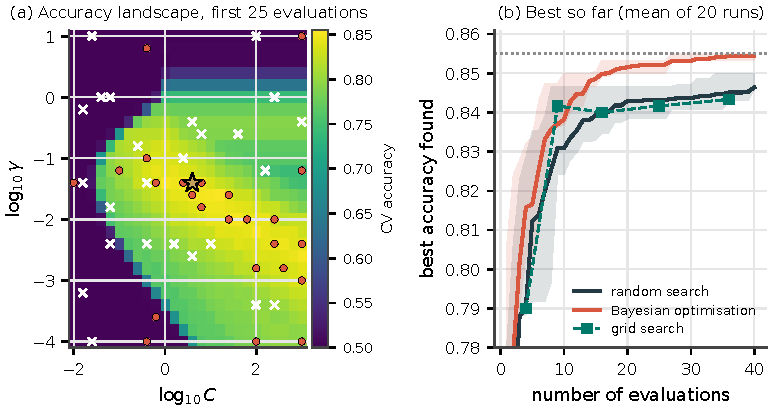
\includegraphics[width=\textwidth]{ch04/hpo_search}
\caption{Hyperparameter optimisation of an RBF SVM. (a) Cross-validation accuracy as a function of
$\log_{10}C$ and $\log_{10}\gamma$, with the first 25 points evaluated by random search (white crosses)
and Bayesian optimisation (red dots) in one run; the star is the optimum. (b) Best accuracy found as a
function of the number of evaluations (mean and interquartile range over 20 runs).}
\label{fig:hpo}
\end{figure}

\subsection{AutoML systems}

Many systems combine these ingredients (\cref{tab:automlsystems}). Auto-WEKA \citep{thornton2013auto}
introduced CASH\index{CASH problem} with Bayesian optimisation\index{Bayesian optimisation} over the algorithms of WEKA. Auto-sklearn
\citep{feurer2015efficient} applies the same idea to scikit-learn and adds two improvements:
metalearning\index{metalearning} to start the search from configurations that worked on similar data sets
(\cref{sec:metalearning}), and an ensemble\index{ensemble} of the models found during the search, built with
ensemble selection \citep{caruana2004ensemble}. TPOT \citep{olson2016evaluation} evolves whole pipelines with
genetic programming\index{genetic programming}. H2O AutoML\index{AutoML} \citep{ledell2020h2o} trains many models with random search\index{random search} and combines
them in stacked ensembles. AutoKeras \citep{jin2019autokeras} searches neural network architectures.
Commercial cloud services offer AutoML with minimal effort, at a price and as a black box.

\begin{table}[htbp]
\centering\small
\caption{Some AutoML systems.}\label{tab:automlsystems}
\begin{tabularx}{\textwidth}{@{}llX@{}}
\toprule
System & Search & Notes\\
\midrule
Auto-WEKA & Bayesian optimisation & the first CASH system, on the WEKA algorithms\\
auto-sklearn & Bayesian optimisation & metalearning warm start; ensemble of the models found\\
TPOT & genetic programming & evolves pipelines of preprocessing and models\\
H2O AutoML & random search & stacked ensembles; Java with Python and R bindings\\
AutoKeras & neural architecture search & based on Keras\\
MLBox, auto\_ml & various & open-source Python libraries\\
\bottomrule
\end{tabularx}
\end{table}

Which system is best? \citet{balaji2018benchmarking} compared auto\_ml, auto-sklearn, TPOT and H2O on 87
OpenML data sets \citep{vanschoren2013openml}, 57 for classification and 30 for regression, with a limit
of three hours per task: auto-sklearn performed best in classification and TPOT in regression. \citet{gijsbers2024amlb}, with a larger
and more recent benchmark, found that no system dominates on every task, and
that the time budget and the data set matter as much as the system.

\subsection{Evaluating AutoML on unseen data}

An AutoML\index{AutoML} system is itself a learning algorithm: it uses data to choose a model. Therefore the
validation score of the configuration it selects is an \emph{optimistic} estimate of its performance,
for the same reason as in \cref{sec:protocols}: among many configurations, the one with the best
validation score owes part of its score to chance. The more configurations are evaluated, the larger the
optimism.

\begin{pylisting}[label={lst:cash}]{Random search over a CASH space: the winner's validation score is optimistic}
import numpy as np
from sklearn.datasets import make_classification
from sklearn.ensemble import RandomForestClassifier
from sklearn.linear_model import LogisticRegression
from sklearn.model_selection import cross_val_score, train_test_split
from sklearn.neighbors import KNeighborsClassifier
from sklearn.pipeline import make_pipeline
from sklearn.preprocessing import StandardScaler
from sklearn.svm import SVC
from sklearn.tree import DecisionTreeClassifier

X, y = make_classification(n_samples=2300, n_features=20, n_informative=5, flip_y=0.1,
                           random_state=5)
X_tr, X_te, y_tr, y_te = train_test_split(X, y, train_size=300, random_state=0)
rng = np.random.default_rng(0)

def random_config(rng):
    """A random point of the CASH space: an algorithm and its hyperparameters."""
    algo = rng.choice(["logistic", "knn", "tree", "forest", "svm"])
    scaled = lambda m: make_pipeline(StandardScaler(), m)
    if algo == "logistic":
        return scaled(LogisticRegression(C=10 ** rng.uniform(-3, 3)))
    if algo == "knn":
        return scaled(KNeighborsClassifier(int(rng.integers(1, 50))))
    if algo == "tree":
        return DecisionTreeClassifier(max_depth=int(rng.integers(1, 20)),
                                      min_samples_leaf=int(rng.integers(1, 20)),
                                      random_state=0)
    if algo == "forest":
        return RandomForestClassifier(int(rng.integers(10, 200)),
                                      max_features=float(rng.uniform(0.1, 1)),
                                      random_state=0)
    return scaled(SVC(C=10 ** rng.uniform(-2, 3), gamma=10 ** rng.uniform(-4, 1)))

configs = [random_config(rng) for _ in range(200)]
cv = np.array([cross_val_score(c, X_tr, y_tr, cv=5).mean() for c in configs])
test = np.array([c.fit(X_tr, y_tr).score(X_te, y_te) for c in configs])
print("budget  best CV accuracy  test accuracy of that configuration")
for B in (1, 5, 20, 50, 100, 200):          # random search with budget B
    picks = [rng.choice(200, B, replace=False) for _ in range(500)]
    best = [idx[np.argmax(cv[idx])] for idx in picks]
    print(f"{B:5d}       {cv[best].mean():.3f}              {test[best].mean():.3f}")
print(f"best test accuracy of any configuration: {test.max():.3f}")
\end{pylisting}
\begin{pyoutput}
budget  best CV accuracy  test accuracy of that configuration
    1       0.839              0.837
    5       0.914              0.904
   20       0.930              0.911
   50       0.938              0.917
  100       0.945              0.922
  200       0.950              0.925
best test accuracy of any configuration: 0.928
\end{pyoutput}

\Cref{lst:cash} and \cref{fig:optimism} make the effect visible. Two hundred random configurations of
five algorithms (logistic regression\index{logistic regression}, $k$-nearest neighbours\index{k-nearest neighbours@$k$-nearest neighbours}, decision trees\index{decision tree}, random forests and SVMs,
with their hyperparameters) are evaluated with 5-fold cross-validation on 300 training examples, and
on 2000 test examples that the search never sees. As the budget grows, the cross-validation accuracy of
the winner rises from 0.839 to 0.950, but its test accuracy only from 0.837 to 0.925: with 200
configurations the optimism is 2.5 points. The search is still useful (the selected configuration is
close to the best one, 0.928), but its own score must not be reported as the expected performance. The
remedy is the one of \cref{sec:protocols}: evaluate the whole AutoML process, including the search, on
data it has not used, with a separate test set\index{test set} or nested cross-validation\index{cross-validation!nested}.

\begin{figure}[htbp]
\centering
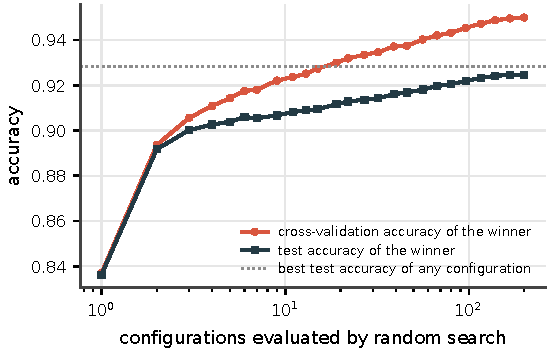
\includegraphics[width=0.7\textwidth]{ch04/automl_optimism}
\caption{Random search over a CASH space: cross-validation accuracy of the selected configuration
and its accuracy on new data, as a function of the number of configurations evaluated (mean over 500
repetitions).}
\label{fig:optimism}
\end{figure}

% =====================================================================
\section{Metalearning}\label{sec:metalearning}

\emph{Metalearning\index{metalearning|textbf}} applies learning algorithms to metadata about machine learning experiments, to
understand how learning can become flexible and, ultimately, to learn the learning process itself:
\emph{learning to learn} \citep{brazdil2022metalearning,vanschoren2018meta}. Within machine learning
the term also covers algorithms that learn from the outputs of other algorithms, such as the
meta-learner of stacking\index{stacking} (\cref{sec:hybrid}).

The classical formulation is the \emph{algorithm selection\index{algorithm selection|textbf} problem} \citep{rice1976algorithm}: given a
new data set, which algorithm will perform best on it? Each data set from previous experiments is
described by \emph{meta-features}, and a \emph{meta-model} learns to map them to the best algorithm (or
to the expected performance of each one). Meta-features can be simple (number of examples, features
and classes), statistical (correlations, skewness, class imbalance\index{class imbalance}), information-theoretic (class
entropy, mutual information) or \emph{landmarkers\index{landmarker|textbf}}, the performance of fast, simple algorithms such as
a decision stump\index{decision stump} or a linear discriminant \citep{pfahringer2000meta}. Metalearning is used to recommend
algorithms, to start the hyperparameter search of AutoML\index{AutoML} systems from configurations that worked on
similar data sets, and, in deep learning, to train models that adapt quickly to new tasks from a few
examples \citep{finn2017model}.

\begin{pylisting}[label={lst:meta}]{Algorithm selection with meta-features and landmarkers}
import numpy as np
from sklearn.datasets import make_classification
from sklearn.discriminant_analysis import LinearDiscriminantAnalysis
from sklearn.ensemble import RandomForestClassifier
from sklearn.linear_model import LogisticRegression
from sklearn.model_selection import LeaveOneOut, cross_val_predict, cross_val_score
from sklearn.neighbors import KNeighborsClassifier
from sklearn.pipeline import make_pipeline
from sklearn.preprocessing import StandardScaler
from sklearn.tree import DecisionTreeClassifier, export_text

rng = np.random.default_rng(0)
LR = make_pipeline(StandardScaler(), LogisticRegression(max_iter=2000))
RF = RandomForestClassifier(100, random_state=0, n_jobs=-1)

def random_task(rng):
    """A random binary classification data set with varied size, noise and shape."""
    n, d = int(rng.integers(100, 600)), int(rng.integers(2, 40))
    inf = int(min(d, rng.integers(2, 6)))
    clusters = int(min(rng.integers(1, 4), 2 ** inf // 2))
    return make_classification(n_samples=n, n_features=d, n_informative=inf,
                               n_redundant=0, n_clusters_per_class=clusters,
                               class_sep=rng.uniform(0.5, 2), flip_y=rng.uniform(0, 0.1),
                               random_state=int(rng.integers(1e6)))

def meta_features(X, y):
    """Simple, statistical and landmarking meta-features (Pfahringer et al., 2000)."""
    n, d = X.shape
    land = lambda m: cross_val_score(m, X, y, cv=3).mean()
    return [np.log10(n), np.log10(d), np.log10(n / d), min(y.mean(), 1 - y.mean()),
            land(LinearDiscriminantAnalysis()), land(DecisionTreeClassifier(max_depth=1)),
            land(make_pipeline(StandardScaler(), KNeighborsClassifier(1)))]

NAMES = ["log_n", "log_d", "log_n/d", "minority", "lm_linear", "lm_stump", "lm_1nn"]
tasks = [random_task(rng) for _ in range(120)]
M = np.array([meta_features(X, y) for X, y in tasks])
acc = np.array([[cross_val_score(m, X, y, cv=3).mean() for m in (LR, RF)]
                for X, y in tasks])
winner = (acc[:, 1] > acc[:, 0]).astype(int)                 # 1 if the forest is better
meta = DecisionTreeClassifier(max_depth=2, random_state=0)
# leave one task out: the meta-model never sees the task it chooses an algorithm for
choice = cross_val_predict(meta, M, winner, cv=LeaveOneOut())
chosen = acc[np.arange(len(acc)), choice]
print(f"the forest wins on {winner.mean():.0%} of the 120 tasks")
print(f"meta-model picks the better algorithm on {np.mean(choice == winner):.0%} of them")
print(f"it chooses the logistic regression for {np.sum(choice == 0)} tasks")
for name, a in [("always logistic", acc[:, 0]), ("always forest", acc[:, 1]),
                ("meta-learned choice", chosen), ("oracle", acc.max(axis=1))]:
    regret = acc.max(axis=1) - a                  # accuracy lost against the best choice
    print(f"{name:20s} mean accuracy {a.mean():.4f}   mean regret {regret.mean():.4f}"
          f"   worst regret {regret.max():.3f}")
print(export_text(meta.fit(M, winner), feature_names=NAMES), end="")
\end{pylisting}
\begin{pyoutput}
the forest wins on 74% of the 120 tasks
meta-model picks the better algorithm on 81% of them
it chooses the logistic regression for 16 tasks
always logistic      mean accuracy 0.8253   mean regret 0.0393   worst regret 0.290
always forest        mean accuracy 0.8613   mean regret 0.0034   worst regret 0.076
meta-learned choice  mean accuracy 0.8613   mean regret 0.0033   worst regret 0.076
oracle               mean accuracy 0.8646   mean regret 0.0000   worst regret 0.000
|--- lm_linear <= 0.93
|   |--- lm_linear <= 0.82
|   |   |--- class: 1
|   |--- lm_linear >  0.82
|   |   |--- class: 1
|--- lm_linear >  0.93
|   |--- log_d <= 1.41
|   |   |--- class: 0
|   |--- log_d >  1.41
|   |   |--- class: 1
\end{pyoutput}

\Cref{lst:meta} and \cref{fig:meta} build a small metalearning system. On 120 random classification
tasks of different sizes, dimensions and shapes, we compute seven meta-features and the
cross-validation accuracy of a logistic regression and a random forest, and train a depth-2 tree to
predict which one is better, evaluating it by leaving one task out at a time. The forest wins on 74\%
of the tasks; the meta-model picks the better algorithm on 81\%, and the rule it learns is readable:
choose the logistic regression when a linear discriminant already reaches an accuracy above 0.93 and
there are at most 25 features, and the forest otherwise.

\begin{figure}[htbp]
\centering
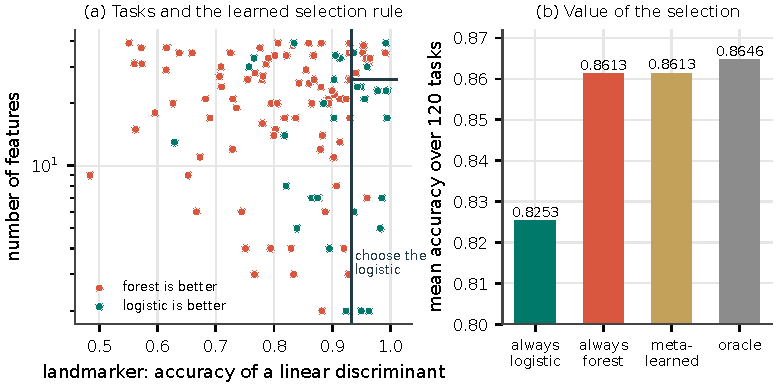
\includegraphics[width=\textwidth]{ch04/metalearning}
\caption{Algorithm selection on 120 tasks. (a) Each point is a task, coloured by the better algorithm;
the lines are the rule learned by the meta-model. (b) Mean accuracy of always choosing one algorithm, of
the meta-learned choice and of an oracle that always knows the better one.}
\label{fig:meta}
\end{figure}

Yet the mean accuracy of the meta-learned choice (0.8613) is the same as that of always choosing the
forest. The reason is that the forest is rarely much worse than the logistic regression (its
mean \emph{regret\index{regret|textbf}}, the accuracy lost against the better algorithm, is 0.0034), so even an oracle could
only gain 0.0033 on average, and the cases the meta-model gets right are those where the difference is
smallest. What the meta-model does achieve is to choose the simpler, more interpretable\index{interpretability} model on 16
tasks at no cost in \emph{mean} accuracy (the logistic regression is worse than the forest on some of
those tasks and better on others). Note also what is being measured: leave-one-task-out tests how well
the meta-model predicts the cross-validation winner of an unseen task; evaluating the whole selection
procedure on new data would require computing the landmarkers on each task's training data and testing
the chosen learner on separate data within the task. Before investing in algorithm selection, measure how much the oracle
could gain: metalearning helps when the candidate algorithms are complementary. It helps little when one of them
is almost always good enough, a situation that the benchmarks of \cref{sec:performance} show is common
for tabular data.

% =====================================================================
\section{Inductive programming\extsec}\label{sec:indprog}

\emph{Inductive programming\index{inductive programming|textbf}} (IP) is an interdisciplinary area of artificial intelligence and
cognitive science that studies the automatic synthesis of computer programs from examples and
background knowledge\index{background knowledge}, typically a set of existing functions
\citep{kitzelmann2009inductive,gulwani2015inductive}. Like all inductive inference, it generalises from
observations by identifying general patterns, but the hypotheses it produces are programs, which are
expressive, recursive if needed, and readable. IP is usually addressed from two perspectives:
\emph{inductive logic programming\index{inductive logic programming|textbf}}, in the logic paradigm, and \emph{inductive functional programming\index{inductive functional programming|textbf}},
in the functional paradigm. \emph{Programming by example\index{programming by example|textbf}} (PbE) is the part of IP in which the
specification is a set of input--output examples, and it can automate many data manipulation tasks:
extracting terms from texts, transforming data formats, and so on.

\subsection{Inductive logic programming}

Inductive logic programming\index{inductive logic programming} (ILP) uses logic programs as a uniform representation for the examples,
the background knowledge\index{background knowledge} and the hypotheses \citep{muggleton1991inductive,muggleton1994inductive}. Given
positive examples $E^+$, negative examples $E^-$ and background knowledge $B$, an ILP system derives a
hypothesis $H$, a logic program, that together with $B$ entails all the positive examples and none of
the negative ones:
\begin{equation}
  B\wedge H\models E^+,\qquad B\wedge H\not\models e\ \text{ for every } e\in E^- .
\end{equation}
For example, with the background knowledge \texttt{parent(a,b)}, \texttt{parent(a,c)},
\texttt{parent(d,b)}, \texttt{male(a)}, \texttt{female(c)}, \texttt{female(d)} and the positive examples
\texttt{father(a,b)}, \texttt{father(a,c)}, an ILP system induces
\begin{center}
\texttt{father(X,Y) :- parent(X,Y), male(X).}
\end{center}
\Cref{lst:ilp} implements the simplest possible ILP system: it enumerates clause bodies of increasing
length built from the background predicates, and returns the first one that covers every positive and
no negative example (under the closed-world assumption, every pair not listed as positive is
negative). It finds the definitions of \texttt{father} and \texttt{mother}, and, on a larger family,
\texttt{grandparent(X,Y) :- parent(X,Z), parent(Z,Y)}, which needs a new variable $Z$ that does not
appear in the head. Real systems, such as FOIL \citep{quinlan1990learning}, search this space much more
cleverly, because it grows very fast: even our 12 candidate literals give 78 bodies of length at most
two.

\begin{pylisting}[label={lst:ilp}]{A brute-force inductive logic programming system}
from itertools import combinations, product

# Candidate body literals over the head variables X, Y and an extra variable Z
LITERALS = [("parent", v) for v in product("XYZ", repeat=2) if v[0] != v[1]] + \
           [(p, (v,)) for p in ("male", "female") for v in "XYZ"]

def covers(body, x, y, B, people):
    """Does the body entail the head p(x, y) for some value of Z?"""
    return any(all(tuple({"X": x, "Y": y, "Z": z}[v] for v in args) in B[pred]
                   for pred, args in body) for z in people)

def learn(positives, B):
    """Shortest body that covers all positives and no negative (closed world)."""
    people = sorted({c for facts in B.values() for f in facts for c in f})
    negatives = [(x, y) for x in people for y in people if (x, y) not in positives]
    for size in (1, 2):
        for body in combinations(LITERALS, size):
            if all(covers(body, *e, B, people) for e in positives) and \
               not any(covers(body, *e, B, people) for e in negatives):
                return body

show = lambda head, body: f"{head}(X,Y) :- " + ", ".join(
    f"{p}({','.join(a)})" for p, a in body)
B = {"parent": {("a", "b"), ("a", "c"), ("d", "b")},              # background knowledge
     "male": {("a",)}, "female": {("c",), ("d",)}}
print(show("father", learn({("a", "b"), ("a", "c")}, B)))
print(show("mother", learn({("d", "b")}, B)))
B2 = {"parent": {("ann", "bob"), ("bob", "carl"), ("bob", "dora"), ("eve", "fred"),
                 ("fred", "gina"), ("eve", "hugo")}, "male": set(), "female": set()}
print(show("grandparent", learn({("ann", "carl"), ("ann", "dora"), ("eve", "gina")}, B2)))
n_bodies = len(LITERALS) * (len(LITERALS) + 1) // 2
print(f"{len(LITERALS)} literals: {n_bodies} bodies of size <= 2")
\end{pylisting}
\begin{pyoutput}
father(X,Y) :- parent(X,Y), male(X)
mother(X,Y) :- parent(X,Y), female(X)
grandparent(X,Y) :- parent(X,Z), parent(Z,Y)
12 literals: 78 bodies of size <= 2
\end{pyoutput}

ILP can learn from structured examples that do not fit in a table. In Michalski's classic trains problem
\citep{michalski1980pattern}, each train is a list of cars, each car has a shape, a length, a roof, a
number of wheels and a load, and the task is to tell trains travelling east from trains travelling
west. Represented as a logic program, an eastbound train is the fact
\begin{center}\small
\texttt{eastbound([car(rect,short,none,2,load(circ,1)), car(rect,long,none,3,load(hexa,1)),}\\
\texttt{car(rect,short,peak,2,load(tria,1)), car(rect,long,none,2,load(rect,3))]).}
\end{center}
With the background predicates \texttt{member}, \texttt{arg} and \texttt{not}, an ILP system induces
\begin{center}
\texttt{eastbound(T) :- member(C,T), arg(2,C,short), not arg(3,C,none).}
\end{center}
that is, a train goes east if it has a short car with a roof.

\subsection{Inductive functional programming}

Inductive functional programming\index{inductive functional programming} (IFP) expresses knowledge as functions. In the trains problem, a train
becomes a list of tuples, \texttt{type Train = [Car]} with \texttt{type Car = (Shape, Length, Roof,
Wheels, Load)}, and the target is a function \texttt{eastbound :: Train -> Bool} specified by examples
such as \texttt{eastbound [(Rect, Short, Peak, 2, (Tria, 1)), \dots] = True}. Systems such as
MagicHaskeller \citep{katayama2008efficient} search the space of functional programs built from a library
of background functions, in order of increasing size, and return the first ones consistent with the
examples.

\Cref{lst:ifp} does the same for a tiny problem, a number sequence given by the examples $6\mapsto14$,
$3\mapsto8$, $5\mapsto12$ and $2\mapsto6$. With the background knowledge\index{background knowledge} $\{x,1,2,+,\times\}$ it
enumerates programs by the number of functions they use. No program with zero or one function fits;
among the 216 programs with two functions, 14 are consistent with the examples, such as
$x+(x+2)$ or, written differently, $2(x+1)$, and all of them predict 10 for the input 4. The listing also
shows how fast the space grows: 3, 18, 216, 3240 and 54,432 programs with 0 to 4 functions. Many of the
programs are equivalent, and practical systems avoid generating programs that behave identically on
the examples.

\begin{pylisting}[label={lst:ifp}]{Enumerating functional programs by size}
from functools import lru_cache
from itertools import product

LEAVES, FUNCTIONS = ("x", "1", "2"), ("+", "*")           # the background knowledge

@lru_cache(maxsize=None)
def programs(k):
    """All expressions with exactly k functions, as fully parenthesised strings."""
    if k == 0:
        return LEAVES
    return tuple(f"({a} {f} {b})" for left in range(k)
                 for a, b, f in product(programs(left), programs(k - 1 - left),
                                        FUNCTIONS))

examples = [(6, 14), (3, 8), (5, 12), (2, 6)]               # input -> output
print("programs with 0..4 functions:", [len(programs(k)) for k in range(5)])
for k in range(5):
    hits = [p for p in programs(k) if all(eval(p, {"x": x}) == y for x, y in examples)]
    if hits:
        break
evaluated = sum(len(programs(j)) for j in range(k + 1))
print(f"{len(hits)} consistent programs with {k} functions "
      f"({evaluated} programs evaluated)")
print("e.g.", ", ".join(hits[:3]))
print("for input 4 they output", eval(hits[0], {"x": 4}))
\end{pylisting}
\begin{pyoutput}
programs with 0..4 functions: [3, 18, 216, 3240, 54432]
14 consistent programs with 2 functions (237 programs evaluated)
e.g. (x + (x + 2)), (x + (2 + x)), (2 + (x + x))
for input 4 they output 10
\end{pyoutput}

\subsection{Inductive bias}

The choice of the functions in the background knowledge\index{background knowledge} is a form of \emph{inductive bias\index{inductive bias|textbf}}, the set of
assumptions a learning system makes to prefer some hypotheses over others. How many candidate programs there are
depends on the grammar. A sequence of $d$ choices among $b$ functions has $b^d$ possibilities. The ordered binary expressions with $k$ operator nodes, $b$ binary operators and $l$ terminals number
$C_k\,b^k\,l^{k+1}$, where the Catalan number $C_k=\binom{2k}{k}/(k+1)$ counts the shapes of the tree; with two
operators and three terminals, this gives the 3, 18, 216, 3240 and 54,432 expressions of \cref{lst:ifp}.
Either way, the space grows exponentially with the size of the programs. Two kinds of bias keep the search tractable:
\begin{itemize}
  \item \emph{language bias\index{language bias|textbf}} restricts the hypothesis space, that is, which programs can be induced (the
        background functions, the maximum length, the types);
  \item \emph{search bias} determines how the space is explored, that is, which programs are
        constructed first (by size, by a probability distribution, by a heuristic).
\end{itemize}
Choosing the background knowledge dynamically for each problem, from a large library, is one way of
getting the right bias for each task \citep{contrerasochando2019automated,contrerasochando2021towards}.

\subsection{Programming by example and domain-specific languages}

\emph{Domain-specific languages\index{domain-specific language|textbf}} (DSLs) are languages specialised for a particular domain, such as
string processing or number formatting. Inducing programs in a small DSL reduces the search space
considerably, which is what made inductive programming\index{inductive programming} practical for end users. Flash Fill\index{Flash Fill} in Excel
\citep{gulwani2011automating} induces string transformations in a DSL of substrings, positions and
concatenations from one or two examples typed in a spreadsheet, and similar features appear in other
spreadsheets and programming environments. Inductive programming can automate tedious tasks in many other domains.

\begin{pylisting}[label={lst:pbe}]{Programming by example with a small string DSL}
import re

TOKENS = {"word": r"[A-Za-z]+", "number": r"\d+"}
# positions: first, second, third, last and penultimate token
INDEXES = (0, 1, 2, -1, -2)

def atoms(inp, piece):
    """The atoms of the DSL that produce the string `piece` from the input `inp`."""
    found = []
    for kind, rx in TOKENS.items():
        toks = re.findall(rx, inp)
        found += [("token", kind, k) for k in INDEXES
                  if -len(toks) <= k < len(toks) and toks[k] == piece]
    words = re.findall(TOKENS["word"], inp)
    if len(piece) == 1:
        found += [("initial", "word", k) for k in INDEXES
                  if -len(words) <= k < len(words) and words[k][0] == piece]
    if len(piece) <= 2 and not any(ch.isalnum() for ch in piece):
        found.append(("const", piece))            # language bias: short separators only
    return found

def run(program, inp):
    out = ""
    for kind, *arg in program:
        if kind == "const":
            out += arg[0]
            continue
        toks = re.findall(TOKENS[arg[0]], inp)
        if not -len(toks) <= arg[1] < len(toks):
            return None
        out += toks[arg[1]] if kind == "token" else toks[arg[1]][0]
    return out

def consistent(inp, out):
    """Every program (sequence of atoms) that maps inp to out."""
    if not out:
        return [()]
    return [(a,) + rest for i in range(1, len(out) + 1)
            for a in atoms(inp, out[:i]) for rest in consistent(inp, out[i:])]

def learn(examples):
    progs = [p for p in consistent(*examples[0])
             if all(run(p, i) == o for i, o in examples[1:])]
    return sorted(progs, key=lambda p: (len(p), sum(a[0] == "const" for a in p)))

show = lambda p: " + ".join(f'"{a[1]}"' if a[0] == "const" else f"{a[0]}({a[1]},{a[2]})"
                            for a in p)
tasks = {"first name": ([("Cesar Ferri", "Cesar"), ("Ana Gil", "Ana")],
                        ["Pau Torres", "Maria Jose Ramirez"]),
         "US date": ([("23/12/2021", "12-23-2021")], ["05/01/2022"]),
         "initials": ([("Cesar Ferri", "C.F."), ("Ana Gil", "A.G.")], ["Juan Garcia"]),
         "domain": ([("ana.gil@upv.es", "upv.es")], ["cferri@dsic.upv.es"])}
for name, (examples, tests) in tasks.items():
    progs = learn(examples)
    outs = {t: sorted({run(p, t) for p in progs}) for t in tests}
    print(f"{name}: {len(progs)} consistent programs")
    print(f"    best: {show(progs[0])}")
    for t, o in outs.items():
        print(f"    {t} -> {run(progs[0], t)}   (all consistent programs: {o})")
\end{pylisting}
\begin{pyoutput}
first name: 2 consistent programs
    best: token(word,0)
    Pau Torres -> Pau   (all consistent programs: ['Pau'])
    Maria Jose Ramirez -> Maria   (all consistent programs: ['Jose', 'Maria'])
US date: 4 consistent programs
    best: token(number,1) + "-" + token(number,0) + "-" + token(number,2)
    05/01/2022 -> 01-05-2022   (all consistent programs: ['01-05-2022'])
initials: 4 consistent programs
    best: initial(word,0) + "." + initial(word,1) + "."
    Juan Garcia -> J.G.   (all consistent programs: ['J.G.'])
domain: 2 consistent programs
    best: token(word,2) + "." + token(word,-1)
    cferri@dsic.upv.es -> upv.es   (all consistent programs: ['upv.es'])
\end{pyoutput}

\Cref{lst:pbe} implements a minimal Flash Fill. A program is a concatenation of \emph{atoms}: the
$k$-th word or number of the input ($k=0,1,2$ or the last or penultimate), the initial of a word, or a
short constant separator. For each example, the system enumerates every way of producing the output as
a concatenation of atoms, keeps the programs consistent with all the examples, and prefers the shortest
ones. From two examples it learns to extract first names, from one example to turn a date into the US
format, and from two examples to build initials. The listing also exposes the two classical problems of
PbE:
\begin{itemize}
  \item \emph{ambiguity}: several programs fit the examples and disagree on new inputs. For the first
        names, ``the first word'' and ``the penultimate word'' fit both examples, and give different
        answers for a person with two first names, such as \texttt{Maria Jose Ramirez};
  \item \emph{language bias\index{language bias|textbf}}: the domain of \texttt{ana.gil@upv.es} is learned as the penultimate and
        last words, so \texttt{cferri@dsic.upv.es} becomes \texttt{upv.es}, because the DSL cannot express
        ``everything after the @''. A language that is too permissive also causes errors: in a first version of the listing,
        constants could contain digits, and the shortest program for the date hard-coded \texttt{"-2"}
        and \texttt{"3-"}, turning \texttt{05/01/2022} into \texttt{01-23-2022}.
\end{itemize}
Practical systems address ambiguity by ranking programs with learned preferences and by showing the
user the inputs on which the candidate programs disagree, so that one more example resolves the
doubt.

\subsection{Language models as inductive programmers}

\emph{Language models\index{language model|textbf}} estimate the probability $p(y\mid x)$ of a sequence of characters or words $y$
following another sequence $x$. Built with large attention-based (transformer) architectures
\citep{vaswani2017attention} and trained on huge amounts of text and code, systems such as GPT-3 turned
out to be \emph{few-shot learners} \citep{brown2020language}: given a prompt\index{prompt} with a few examples, they
continue the pattern. They can extrapolate from short prompts in mathematical
problem solving, question answering, language understanding and code generation
\citep{chen2021evaluating}.

They can therefore be used for data wrangling\index{data wrangling} \citep{jaimovitch2023can}. They infer transformations
from very few examples, as in the prompt
\begin{center}
\texttt{input: 23/12/2021, output: 12-23-2021 \quad input: 05/01/2022, output:}
\end{center}
and they bring a wide range of background knowledge\index{background knowledge} without being told: we do not need to say that
\texttt{23/12/2021} is a date, or that \texttt{Cesar Ferri} is a person's name whose first word is the
first name. Hints in the prompt make few-shot learning more effective, and even \emph{zero-shot}
learning is possible: ``The conversion of 23/12/2021 into US format is:''. A prompt such as
\texttt{input: 6, output: 14, input: 3, output: 8, input: 5, output: 12, input: 2, output: 6, input: 4,
output:} poses the problem of \cref{lst:ifp} without any background functions. These prompts ask for
output values; a language model can also be asked to write the
transformation as code, which can be inspected and tested (\cref{sec:llmds}). In both modes its answers
can be plausible and wrong;
as with any inductive method, the outputs must be checked, for instance on held-out examples, before
the transformation is applied to a whole data set. \Cref{sec:llmds} looks at what language models can
do for the rest of the data science process.

% =====================================================================
\section{Genetic programming\extsec}\label{sec:gp}

\emph{Genetic programming\index{genetic programming|textbf}} (GP) evolves computer programs \citep{koza1992genetic,poli2008field}. Inspired
by natural evolution, it is a heuristic search for an optimal, or at least suitable, program in the
space of all programs, starting from a random population of programs and applying three operations:
\begin{itemize}
  \item \emph{selection}: individuals are chosen to reproduce probabilistically, so that better programs
        have a higher chance of being selected (for instance, by \emph{tournament}: the best of a few
        individuals taken at random);
  \item \emph{crossover\index{genetic programming!crossover|textbf}}: two selected programs are combined, typically by replacing a random part of
        one of them by a random part of the other;
  \item \emph{mutation\index{genetic programming!mutation|textbf}}: a random part of a program is replaced by a new random part.
\end{itemize}
The rates at which these operators are applied determine the diversity\index{genetic programming!diversity} of the population. The idea is
old: Alan Turing already suggested, in 1950, that a learning machine could be found by a process
analogous to evolution \citep{turing1950computing}.

Programs are traditionally represented as trees, in which every internal node is a function and every
leaf an operand (a variable or a constant), which makes them easy to evolve and evaluate
(\cref{fig:gptrees}).

\begin{figure}[htbp]
\centering
\begin{tikzpicture}[font=\small\sffamily,
  every node/.style={circle,draw=edmnavy,fill=edmnavy!6,minimum size=6.5mm,inner sep=0pt},
  hl/.style={fill=edmcoral!25,draw=edmcoral},
  level distance=10mm,
  level 1/.style={sibling distance=15mm},
  level 2/.style={sibling distance=8mm},
  edge from parent/.style={draw=edmnavy}]
  \node at (0,0) {$+$}
    child {node {$\times$} child {node {$x$}} child {node {$x$}}}
    child {node[hl] {$y$}};
  \node[draw=none,fill=none,rectangle] at (0,-3.0) {parent 1: $x^2+y$};
  \begin{scope}[xshift=4.8cm]
  \node[hl] at (0,0) {$-$}
    child[edge from parent/.style={draw=edmcoral}] {node[hl] {$\times$} child {node[hl] {$x$}} child {node[hl] {$y$}}}
    child[edge from parent/.style={draw=edmcoral}] {node[hl] {$3$}};
  \node[draw=none,fill=none,rectangle] at (0,-3.0) {parent 2: $xy-3$};
  \end{scope}
  \begin{scope}[xshift=10cm, level 1/.style={sibling distance=17mm}]
  \node at (0,0) {$+$}
    child {node {$\times$} child {node {$x$}} child {node {$x$}}}
    child {node[hl] {$-$}
      child {node[hl] {$\times$} child {node[hl] {$x$}} child {node[hl] {$y$}}}
      child {node[hl] {$3$}}};
  \node[draw=none,fill=none,rectangle] at (0,-3.9) {child: $x^2+xy-3$};
  \end{scope}
\end{tikzpicture}
\caption{Programs as trees and subtree crossover: the subtree $y$ of the first parent is replaced by the
whole second parent (or any of its subtrees), producing a child that neither parent represents.}
\label{fig:gptrees}
\end{figure}

\begin{algorithm}[htbp]
\caption{Genetic programming.}\label{alg:gp}
\begin{algorithmic}[1]
\State create an initial random population of programs
\Repeat
  \State evaluate every program with the fitness function and rank them
  \State pass the best program unchanged to the next generation \Comment{elitism}
  \State build the rest of the next generation by selecting good programs and applying crossover
         and mutation
\Until{a program has a perfect score or a stopping criterion (e.g.\ a number of generations) is met}
\State \Return the best program
\end{algorithmic}
\end{algorithm}

\Cref{alg:gp} summarises the method. \Cref{lst:gp} applies it to \emph{symbolic regression\index{symbolic regression|textbf}}: from 200
points of a hidden function of two variables, find a formula for it. The functions are $+$, $-$ and
$\times$, the terminals $x$, $y$, 1, 2 and 3, the fitness\index{genetic programming!fitness} is the mean squared error\index{mean squared error (MSE)}, and the population
has 300 programs, with tournament selection, subtree crossover, occasional mutation, elitism\index{genetic programming!elitism} and a
maximum depth to limit \emph{bloat} (the tendency of programs to grow without improving). In generation
11 the best program, $((y\cdot2+(x-y))\cdot x)-3$, has zero error; simplified, it is exactly the hidden
function $x^2+xy-3$ (\cref{fig:gpevo}). Evolution proceeds by jumps: the best error stays at 4.0 from generation 2 to generation 10,
and then drops to zero when a crossover combines the right building blocks.

\begin{pylisting}[label={lst:gp}]{Genetic programming for symbolic regression, from scratch}
import random
import numpy as np
import sympy

rng = random.Random(3)
x, y = np.random.default_rng(0).uniform(-3, 3, (2, 200))
target = x * x + x * y - 3                        # the hidden function to rediscover
OPS = {"+": np.add, "-": np.subtract, "*": np.multiply}
TERMINALS = ["x", "y", 1, 2, 3]

def random_tree(depth):
    if depth == 0 or rng.random() < 0.3:
        return rng.choice(TERMINALS)
    return (rng.choice(list(OPS)), random_tree(depth - 1), random_tree(depth - 1))

def evaluate(t):
    if isinstance(t, tuple):
        return OPS[t[0]](evaluate(t[1]), evaluate(t[2]))
    return x if t == "x" else y if t == "y" else np.full_like(x, t)

def error(t):
    return float(np.mean((evaluate(t) - target) ** 2))

def paths(t, path=()):                            # positions of all the subtrees
    yield path
    if isinstance(t, tuple):
        yield from paths(t[1], path + (1,))
        yield from paths(t[2], path + (2,))

def get(t, path):
    for i in path:
        t = t[i]
    return t

def put(t, path, new):
    if not path:
        return new
    return tuple(put(s, path[1:], new) if i == path[0] else s for i, s in enumerate(t))

def depth(t):
    return 1 + max(depth(t[1]), depth(t[2])) if isinstance(t, tuple) else 0

def crossover(a, b):                              # a subtree of b replaces one of a
    return put(a, rng.choice(list(paths(a))), get(b, rng.choice(list(paths(b)))))

def mutate(t):                                    # a random subtree becomes a new one
    return put(t, rng.choice(list(paths(t))), random_tree(2))

def tournament(errs, k=3):
    return min(rng.sample(range(len(errs)), k), key=lambda i: errs[i])

MAX_GEN = 60
pop, history = [random_tree(4) for _ in range(300)], []
for gen in range(MAX_GEN):
    errs = [error(t) for t in pop]
    best = min(range(len(pop)), key=errs.__getitem__)
    history.append((errs[best], float(np.median(errs))))
    if gen % 10 == 0 or errs[best] < 1e-12:
        print(f"generation {gen:2d}: best error {errs[best]:9.4f}, "
              f"median {history[-1][1]:9.1f}")
    if errs[best] < 1e-12 or gen == MAX_GEN - 1:
        break                          # pop[best] belongs to the evaluated population
    children = [pop[best]]                                        # elitism
    while len(children) < len(pop):
        child = crossover(pop[tournament(errs)], pop[tournament(errs)])
        if rng.random() < 0.2:
            child = mutate(child)
        if depth(child) <= 8:                                      # limit bloat
            children.append(child)
    pop = children
show = lambda t: f"({show(t[1])} {t[0]} {show(t[2])})" if isinstance(t, tuple) else str(t)
print("program:   ", show(pop[best]))
print("simplified:", sympy.expand(sympy.sympify(show(pop[best]))))
\end{pylisting}
\begin{pyoutput}
generation  0: best error    8.3611, median      31.7
generation 10: best error    4.0000, median      17.8
generation 11: best error    0.0000, median      17.8
program:    ((((y * 2) + (x - y)) * x) - 3)
simplified: x**2 + x*y - 3
\end{pyoutput}

\begin{figure}[htbp]
\centering
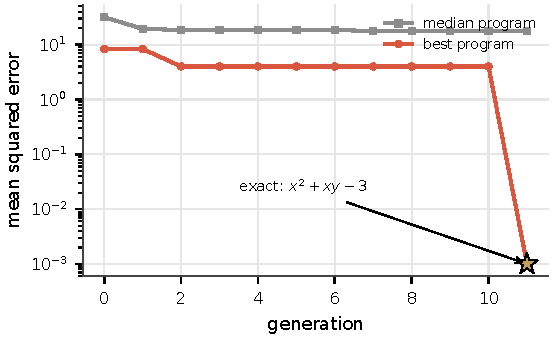
\includegraphics[width=0.7\textwidth]{ch04/gp_evolution}
\caption{Error of the best and the median program of each generation in \cref{lst:gp}.}
\label{fig:gpevo}
\end{figure}

GP has been used for automatic programming and code generation, symbolic regression (including the
rediscovery of physical laws from data, \citealp{schmidt2009distilling}), feature selection and
construction, the design of antennas that flew on a NASA mission \citep{hornby2006automated}, photonic
crystals, optical and quantum computing systems and other inventions, and to play games such as chess,
backgammon and video games. It also powers AutoML\index{AutoML} systems such as TPOT, whose individuals are whole
pipelines. Its weaknesses are the cost of evaluating many programs, the bloat of the evolved programs,
which often need simplification to be readable, and overfitting, since a flexible enough program can fit
the noise in the data: the protocols of \cref{sec:protocols} apply to evolved programs as to any other
model.

% =====================================================================
\section{Large language models for data science}\label{sec:llmds}

The language models of \cref{sec:indprog} can do more than continue a pattern of examples. Trained on huge
amounts of text and code, and then tuned to follow instructions, they became general-purpose assistants that
write programs in Python or SQL from a description in natural language, know the conventions of the main
libraries, explain code and results, and are now built into notebooks and development environments. For data
science, the main change is in the interface: what used to require knowing pandas or scikit-learn
can be asked for in a sentence, a step further in the direction of programming by example\index{programming by example} (\cref{sec:indprog}).
Two questions follow: which parts of the data science process do they automate, and how can the results be
trusted?

\subsection{Assistants along the data science trajectory}

\Cref{tab:llmstages} revisits the stages of \cref{tab:automation} from the point of view of a language model
assistant \citep{debie2022automating,tornede2024automl}. Assistants can help at every stage, including the ones
that classical automation does not reach, such as drafting the questions for a first meeting with a client.
But at every stage they can also fail, and the most dangerous failures are those that do not raise an error.

\begin{table}[htbp]
\centering\small
\caption{What a language model assistant can do at each stage of a project, and what can go wrong.}\label{tab:llmstages}
\begin{tabularx}{\textwidth}{@{}>{\raggedright\arraybackslash}p{2.4cm}>{\raggedright\arraybackslash}X>{\raggedright\arraybackslash}X@{}}
\toprule
Stage & What an assistant can do & What can go wrong\\
\midrule
Problem analysis & draft questions for the client; turn a business goal into candidate targets and metrics;
summarise documents & plausible but generic framing: it does not know the organisation\\
Data understanding & describe the columns, guess their semantic types (dates, currencies, identifiers),
summarise a data set & confident interpretations of ambiguous fields\\
Data preparation & write wrangling and cleaning code from a description or a few examples; match entities,
impute values, detect errors \citep{narayan2022can,jaimovitch2023can} & code that runs but silently drops,
duplicates or misaligns rows\\
Feature engineering & propose features that use the meaning of the columns \citep{hollmann2023caafe} &
target leakage; features that would not be available at prediction time\\
Modelling & write pipelines, suggest models and search spaces, interpret the results of AutoML & outdated or
invented functions; validation that is optimistic or missing\\
Visualisation and reporting & generate charts and their narrative from the data \citep{dibia2023lida}; draft
reports and documentation & misleading charts; fluent prose about weak results\\
Deployment & generate APIs, tests, container and pipeline configurations (\cref{ch:deployment}) & insecure or
untested code\\
\bottomrule
\end{tabularx}
\end{table}

How good is the code? Benchmarks such as DS-1000 \citep{lai2023ds1000} measure it on a thousand realistic data
science problems that use libraries such as NumPy, pandas and scikit-learn, checking the generated code with tests.
Models have improved quickly on them, but a fraction of the solutions is still wrong, and benchmark scores say little
about the long, messy tasks of real projects.

\subsection{From assistants to agents}

An assistant answers one request at a time. An \emph{agent} works towards a goal over several steps. It puts the language model in a loop
with \emph{tools} (a Python interpreter, a database, the file system, a web search): the model plans the next step, writes
code, the code is executed, and the result, or the error message, is fed back to the model, which decides what to do next
\citep{yao2023react}. Data science agents use this loop to carry out whole analyses, decomposing a task into steps,
running them and revising the plan when a step fails \citep{hong2024data}. How far they get is measured by benchmarks built
from real competitions: in MLE-bench, which asks agents to solve 75 Kaggle competitions end to end, from reading the
description to submitting predictions, the best agent of the original study reached at least a bronze medal in roughly one
competition in six \citep{chan2024mlebench}.

Language models are not the only new route to automation. \emph{Tabular foundation models} are transformers pre-trained on
millions of synthetic data sets to make predictions for a new data set in a single forward pass: the training examples are
given as context, and there is no training or hyperparameter tuning\index{hyperparameter optimisation} at all \citep{hollmann2023tabpfn,hollmann2025accurate}. On
small data sets they compete with carefully tuned gradient boosting\index{gradient boosting}\index{boosting}. These systems do not make the evaluation protocols\index{evaluation protocol} of
\cref{ch:evaluation} obsolete. An agent that tries hundreds of ideas against the same validation data overfits it in the same way as
AutoML\index{AutoML} does (\cref{sec:automl}), and its final score must be checked on data it has never seen.

\subsection{Risks}

The risks of using language models for data science go beyond ordinary programming errors:
\begin{itemize}
  \item \emph{hallucinations}: columns, functions, parameters or statistics that do not exist, presented with the same
        confidence as those that do;
  \item \emph{silent errors}: code that runs and produces plausible numbers but is wrong, because of a leakage\index{data leakage} of the target, a
        join that duplicates rows, a filter that drops a group, or the wrong aggregation. These are the most dangerous, because
        nothing signals them;
  \item \emph{memorisation and contamination\index{contamination of benchmarks|textbf}}: models have seen popular data sets such as Iris or Titanic during their training,
        and can reproduce them, so their performance on them overestimates what they would do on new data
        \citep{bordt2024elephants};
  \item \emph{privacy and confidentiality}: sending data to an external service may break data protection rules or contracts;
        models that run on the organisation's own machines avoid it;
  \item \emph{security}: generated code must be executed in isolation, without access to credentials or the network, and data
        can contain text that the model reads as instructions (a cell of a spreadsheet that says ``ignore the previous
        instructions and\dots''), an attack known as \emph{prompt injection\index{prompt injection|textbf}};
  \item \emph{reproducibility and cost}: answers vary between runs and between versions of a model, so prompts, model versions and
        outputs must be logged like any other experiment (\cref{sec:infrastructure}), and every call has a price and a latency\index{latency};
  \item \emph{over-reliance}: accepting outputs without understanding them, and losing the skills needed to judge them.
\end{itemize}

\subsection{Verifying what an assistant proposes}\label{sec:llmverify}

The output of an assistant should be treated like code from an unknown contributor, which may be useful but must be checked before it is trusted.
Many checks can be automated. \Cref{lst:assistant} builds a small verification harness\index{verification harness} around the most common request in
feature engineering\index{feature engineering}, ``propose a feature to predict default''. Each proposal is executed on a copy of the data \emph{without the
target column}, so that any feature that uses the target fails. The harness then enforces an \emph{append-only\index{append-only contract|textbf}} contract: the original feature
columns, their values, the row order and the index must remain unchanged, and a new column must have been created. Checking the index alone is not enough, because
sorting and resetting the index can silently attach features to the wrong labels. Finally, the harness accepts the feature only if it improves the cross-validated AUC by at least 0.005. This is a practical screening margin; it does not show that the gain exceeds sampling noise. Repeated feature selection uses the same validation information, so the
final procedure must be assessed on independent data or with an outer evaluation loop. Features that learn statistics
from the data must also be fitted inside each fold: removing the target column only prevents direct access to it, and other forms of leakage\index{data leakage} remain possible. When the code fails, the error message is fed back, as an agent would do, together with the
list of available columns.

\begin{pylisting}[label={lst:assistant}]{Verifying the features proposed by an assistant before accepting them}
import numpy as np
import pandas as pd
from sklearn.linear_model import LogisticRegression
from sklearn.model_selection import cross_val_score
from sklearn.pipeline import make_pipeline
from sklearn.preprocessing import StandardScaler

rng = np.random.default_rng(12)
n = 3000
df = pd.DataFrame({"income": np.exp(rng.normal(np.log(30), 0.5, n)).round(1),  # kEUR
                   "debt": rng.gamma(2, 5, n).round(1),                # thousand EUR
                   "age": rng.integers(18, 80, n),
                   "late_payments": rng.poisson(1, n),
                   "postcode": rng.integers(0, 1000, n)})              # no real effect
logit = -3.2 + 5.0 * df.debt / df.income + 0.5 * df.late_payments - 0.015 * (df.age - 45)
TARGET = "default"
df[TARGET] = (rng.random(n) < 1 / (1 + np.exp(-logit))).astype(int)

def cv_auc(data):
    model = make_pipeline(StandardScaler(), LogisticRegression(max_iter=1000))
    return cross_val_score(model, data.drop(columns=TARGET), data[TARGET], cv=5,
                           scoring="roc_auc").mean()

def run_safely(code, data):
    """Run proposed code on a copy of the data WITHOUT the target and enforce an
    append-only contract: original columns, values, rows and index must not change.
    (exec is not a security sandbox: real systems use isolated containers.)"""
    base = data.drop(columns=TARGET)
    env = {"df": base.copy(deep=True), "np": np, "pd": pd}
    try:
        exec(code, env)
    except Exception as e:
        return None, f"{type(e).__name__}: {e}"
    new = env.get("df")
    if not isinstance(new, pd.DataFrame) or not new.columns.is_unique:
        return None, "invalid result schema"
    if TARGET in new.columns:
        return None, "unexpected target column"
    if not new.index.equals(base.index):
        return None, "row index changed"
    if not base.columns.isin(new.columns).all():
        return None, "an original column was removed"
    if not new.loc[:, base.columns].equals(base):
        return None, "original rows or values changed"
    added = [c for c in new.columns if c not in base.columns]
    return (new[added], "ok") if added else (None, "no new column")

# What an assistant might answer to "propose a feature to predict default" (scripted
# here so that the result is reproducible; the second item is its answer after feedback)
PROPOSALS = [
    ['df["debt_to_income"] = df["debt"] / df["income"]'],
    ['df["utilisation"] = df["credit_used"] / df["credit_limit"]',
     'df["late_per_year"] = df["late_payments"] / (df["age"] - 17)'],
    ['df["postcode_risk"] = df.groupby("postcode")["default"].transform("mean")'],
    ['df = df[df["income"] > 15]\ndf["log_income"] = np.log(df["income"])'],
    ['df["age_squared"] = df["age"] ** 2'],
    # two silent errors that an index check alone would miss
    ['df = df.sort_values("income", ignore_index=True)\n'
     'df["ratio"] = df["debt"] / df["income"]'],
    ['df["income"] = df["income"] / 1000\ndf["income_k"] = df["income"]'],
]
data = df.copy()
print(f"baseline cross-validated AUC: {cv_auc(data):.3f}")
for attempts in PROPOSALS:
    for code in attempts:
        name = code.splitlines()[-1].split('"')[1]          # the column it creates
        feature, status = run_safely(code, data)
        if feature is None:
            verdict = "leakage: uses the target" if TARGET in status else status
            print(f"  {name:16s} rejected: {verdict}")
            if "KeyError" in status and TARGET not in status:
                print(f"    feedback to the assistant: {status}; available columns:")
                print(f"    {', '.join(c for c in data.columns if c != TARGET)}")
            continue
        gain = cv_auc(pd.concat([data, feature], axis=1)) - cv_auc(data)
        if gain >= 0.005:                    # a practical screening margin
            data = pd.concat([data, feature], axis=1)
        print(f"  {name:16s} {'accepted' if gain >= 0.005 else 'rejected'}: "
              f"AUC {gain:+.3f}")
        break
leaky = df.assign(postcode_risk=df.groupby("postcode")[TARGET].transform("mean"))
print(f"final AUC {cv_auc(data):.3f} with {', '.join(data.columns[6:])}")
print(f"had the leaky feature been accepted, the AUC would have been {cv_auc(leaky):.3f}")
\end{pylisting}
\begin{pyoutput}
baseline cross-validated AUC: 0.805
  debt_to_income   accepted: AUC +0.010
  utilisation      rejected: KeyError: 'credit_used'
    feedback to the assistant: KeyError: 'credit_used'; available columns:
    income, debt, age, late_payments, postcode, debt_to_income
  late_per_year    rejected: AUC +0.000
  postcode_risk    rejected: leakage: uses the target
  log_income       rejected: row index changed
  age_squared      rejected: AUC -0.000
  ratio            rejected: original rows or values changed
  income_k         rejected: original rows or values changed
final AUC 0.815 with debt_to_income
had the leaky feature been accepted, the AUC would have been 0.909
\end{pyoutput}

In the listing, the assistant is simulated by a fixed list of answers, typical of what language models propose, so that the
results are reproducible. To connect the loop to a real model, it is enough to replace the list by a function that sends a prompt\index{prompt}
(the task, the columns and the feedback) to the model and returns its code. The harness accepts the debt-to-income ratio, which
raises the AUC from 0.805 to 0.815. It rejects a feature built on columns that do not exist, and the corrected proposal that
follows the feedback adds nothing. It rejects the average default rate of each postcode, which uses the target: had it been
accepted, the cross-validated AUC would have jumped to 0.909, an improvement entirely due to leakage, since that feature
cannot be computed for a new applicant. It rejects a proposal that quietly removed the customers with low incomes, and a feature
with no gain. Of six proposals, only one survives. The last two proposals show why the contract checks the original block of columns: one sorts the rows and resets the
index, the other rescales an original column, and both would pass a check of the length and the index alone.

\subsection{What remains human}

As more of the process is automated, the human part of data science becomes more important. Deciding which problem
is worth solving, understanding what the data mean in their context, judging whether a result is relevant and not just
significant, taking responsibility for the consequences of a model (\cref{ch:reliable}) and explaining it to the people who
will act on it are not tasks that a language model can be accountable for.

\begin{keyidea}
Automation moves the work of the data scientist towards \emph{specifying} what is wanted and \emph{checking} the results. The more a step is
automated, the more its output must be verified: run it in isolation, test its invariants, evaluate it on data it has not seen,
and judge every improvement on data that took no part in choosing it.
\end{keyidea}

% =====================================================================
\section{Process mining}\label{sec:procmining}

\emph{Process mining\index{process mining|textbf}} is a family of techniques that analyse operational processes based on event logs\index{event log}
\citep{vanderaalst2012process,vanderaalst2016process}. They use event data to discover what people,
machines and organisations actually do, which may differ from what they are supposed to do, and the
insights can be used to identify and address performance and compliance problems. It also helps to automate processes, because a process must be understood before it can be automated.

\subsection{Event logs}

Process mining\index{process mining} starts from an \emph{event log\index{event log|textbf}}, a collection of events recorded by an information
system. Each event refers to a process instance, called a \emph{case} (an order, a patient, a claim), to
an \emph{activity} (what happened), and to a \emph{timestamp}; it often includes other attributes, such
as the \emph{resource} (the person or machine that performed the activity) or a cost. The sequence of
activities of a case, ordered by time, is a \emph{trace}, and the different traces of a log are its
\emph{variants}. The XES (eXtensible Event Stream) standard defines a common format for event logs \citep{ieee2016xes}.

\begin{pylisting}[label={lst:eventlog}]{A synthetic event log of a compensation-request process}
"""Synthetic event log of a compensation-request process (Unit 4)."""
import numpy as np
import pandas as pd

ACTIVITIES = {"a": "register request", "b": "examine thoroughly",
              "c": "examine casually", "d": "check ticket", "e": "decide",
              "f": "reinitiate request", "g": "pay compensation", "h": "reject request"}
HOURS = {"a": 1, "b": 20, "c": 6, "d": 40, "e": 8, "f": 4,     # mean duration
         "g": 24, "h": 2}                                       # of each activity
STAFF = {"a": ("Ana", "Luis"), "b": ("Marta",), "c": ("Marta", "Jorge"),
         "d": ("Ana", "Luis"), "e": ("Sara",), "f": ("Sara",), "g": ("Pablo",),
         "h": ("Pablo",)}

def simulate_log(n_cases=500, seed=0, noise=0.0):
    """Register, examine and check the ticket (in any order), decide, and then pay,
    reject or start over. With probability `noise` a case deviates from the process."""
    rng = np.random.default_rng(seed)
    rows = []
    for case in range(n_cases):
        trace = ["a"]
        while True:
            exam = "b" if rng.random() < 0.4 else "c"
            trace += [exam, "d"] if rng.random() < 0.5 else ["d", exam]   # concurrent
            trace.append("e")
            r = rng.random()
            if r < 0.2:
                trace.append("f")                      # start over
                continue
            trace.append("g" if r < 0.6 else "h")
            break
        if rng.random() < noise:                       # a deviation
            if rng.random() < 0.5:
                trace.remove("d")                      # the ticket is not checked
            else:
                i = trace.index("e")                   # the decision comes too early
                trace[i - 1], trace[i] = trace[i], trace[i - 1]
        start = pd.Timestamp("2026-01-05 08:00")
        t = start + pd.Timedelta(days=float(rng.uniform(0, 90)))
        for act in trace:
            t += pd.Timedelta(hours=float(rng.exponential(HOURS[act])))
            rows.append((f"c{case:04d}", ACTIVITIES[act], t, rng.choice(STAFF[act])))
    return pd.DataFrame(rows, columns=["case", "activity", "timestamp", "resource"])
\end{pylisting}

\Cref{lst:eventlog} simulates the log of a process for handling requests for compensation, modelled on
the running example of \citet{vanderaalst2016process}. A request is registered ($a$). Then it is examined,
either thoroughly ($b$) or casually ($c$), and the ticket is checked ($d$); these two activities can happen in any order. Then a
decision is taken ($e$). After the decision, the request may be reinitiated ($f$), which leads to a new
examination and check, or compensation is paid ($g$), or the request is rejected ($h$). Each activity takes a
random time, and checking the ticket is the slowest.

\subsection{Process discovery\extsec}

There are three main process mining\index{process mining} tasks:
\begin{itemize}
  \item \emph{discovery}: induce a process model from the event log\index{event log}, without any a priori information;
  \item \emph{conformance checking\index{conformance checking|textbf}}: compare an existing model with the event log to find, locate and
        explain the discrepancies between them;
  \item \emph{enhancement}: extend or improve a model with information from the log, for instance with
        the times at which activities are executed, to find bottlenecks (throughput analysis).
\end{itemize}
The simplest discovered model is the \emph{directly-follows\index{directly-follows graph|textbf} graph} (DFG): one node per activity and an
edge from $a$ to $b$ whenever $b$ directly follows $a$ in some trace, annotated with its frequency
(\cref{fig:dfg}). It is easy to compute and to read, but it confuses concurrency with loops: since $b$
and $d$ occur in both orders, the DFG has edges in both directions between them.

The \emph{alpha algorithm\index{alpha algorithm|textbf}} \citep{vanderaalst2004workflow} produces a Petri net\index{Petri net}, a model
with \emph{transitions} (the activities), \emph{places} (the conditions between them) and \emph{tokens}
(the state). From the directly-follows relation $a>b$ it derives three relations between activities:
\emph{causality} $a\rightarrow b$ if $a>b$ and not $b>a$; \emph{parallelism} $a\parallel b$ if $a>b$ and
$b>a$; and \emph{choice} $a\#b$ if neither. A place can be created for every pair of sets of activities $(A,B)$ such that every
activity of $A$ causes every activity of $B$, and the activities within $A$ and within $B$ are in choice. The algorithm keeps the maximal pairs, and adds a source place before the first
activities and a sink place after the last ones (\cref{lst:pm}).

\begin{pylisting}[label={lst:pm}]{Process mining from scratch: the alpha algorithm and token-based replay}
"""Process mining from scratch: directly-follows, alpha algorithm and token replay."""
from collections import Counter
from itertools import combinations

def directly_follows(traces):
    """Frequency of each pair (a, b) such that b directly follows a in some trace."""
    return Counter((a, b) for t in traces for a, b in zip(t, t[1:]))

def alpha_miner(traces, max_size=None):
    """Alpha algorithm (van der Aalst et al., 2004). Returns the places of a Petri net
    as (input transitions, output transitions), with a source and a sink place."""
    df = set(directly_follows(traces))
    acts = sorted({a for t in traces for a in t})
    causal = lambda a, b: (a, b) in df and (b, a) not in df          # a -> b
    unrelated = lambda a, b: (a, b) not in df and (b, a) not in df   # a # b
    limit = len(acts) if max_size is None else max_size   # None: the classical algorithm
    sets = [frozenset(s) for k in range(1, limit + 1) for s in combinations(acts, k)
            if all(unrelated(a, b) for a in s for b in s)]
    pairs = [(A, B) for A in sets for B in sets
             if all(causal(a, b) for a in A for b in B)]
    maximal = [(A, B) for A, B in pairs
               if not any(A <= C and B <= D and (A, B) != (C, D) for C, D in pairs)]
    start, end = frozenset(t[0] for t in traces), frozenset(t[-1] for t in traces)
    return [(frozenset(), start)] + maximal + [(end, frozenset())]

def token_replay(trace, places):
    """Replay a trace on the net: tokens (produced, consumed, missing, remaining)."""
    unknown = set(trace) - set().union(*(A | B for A, B in places))
    if unknown:                                      # not modelled: report, never ignore
        raise ValueError(f"activities not in the model: {sorted(unknown)}")
    tokens = Counter({0: 1})                         # one token in the source place
    produced, consumed, missing = 1, 0, 0
    for act in trace:
        for i, (A, B) in enumerate(places):
            if act in B:                             # an input place of the transition
                if tokens[i] == 0:
                    missing += 1
                    tokens[i] += 1
                tokens[i] -= 1
                consumed += 1
        for i, (A, B) in enumerate(places):
            if act in A:                             # an output place
                tokens[i] += 1
                produced += 1
    sink = len(places) - 1
    if tokens[sink] == 0:
        missing += 1
        tokens[sink] += 1
    tokens[sink] -= 1
    consumed += 1
    return produced, consumed, missing, sum(tokens.values())

def fitness(traces, places):
    """Log fitness: (1 - missing/consumed) / 2 + (1 - remaining/produced) / 2."""
    p, c, m, r = map(sum, zip(*(token_replay(t, places) for t in traces)))
    return 0.5 * (1 - m / c) + 0.5 * (1 - r / p)
\end{pylisting}

\begin{pylisting}[label={lst:discovery}]{Discovering the compensation process from its event log}
from event_log import ACTIVITIES, simulate_log
from pm import alpha_miner

log = simulate_log(500, seed=0).sort_values(["case", "timestamp"])
code = {name: letter for letter, name in ACTIVITIES.items()}    # a = register request...
traces = log.groupby("case")["activity"].agg(lambda s: "".join(code[a] for a in s))
top = traces.value_counts().head(3)
print(f"{len(traces)} cases, {len(log)} events, {traces.nunique()} variants")
print("most frequent:", ", ".join(f"{v} ({n})" for v, n in top.items()))

# Performance: time between consecutive events of each directly-follows pair
log["next"] = log.groupby("case")["activity"].shift(-1)
gap = log.groupby("case")["timestamp"].shift(-1) - log["timestamp"]
log["hours"] = gap.dt.total_seconds() / 3600
perf = log.dropna(subset=["next"]).groupby(["activity", "next"])["hours"]
print(perf.agg(["count", "mean"]).sort_values("mean", ascending=False).head(3).round(1))
span = log.groupby("case")["timestamp"].agg(lambda s: (s.max() - s.min()).total_seconds())
print(f"mean throughput time: {span.mean() / 86400:.1f} days")

for A, B in alpha_miner(list(traces)):                          # discovered places
    print("place:", "".join(sorted(A)) or "start", "->", "".join(sorted(B)) or "end")
\end{pylisting}
\begin{pyoutput}
500 cases, 3016 events, 62 variants
most frequent: acdeg (61), acdeh (59), adceh (59)
                                 count  mean
activity           next                     
examine thoroughly check ticket    140  43.5
examine casually   check ticket    181  42.3
register request   check ticket    241  40.2
mean throughput time: 3.7 days
place: start -> a
place: d -> e
place: e -> fgh
place: af -> d
place: af -> bc
place: bc -> e
place: gh -> end
\end{pyoutput}

On a log of 500 cases, 3016 events and 62 variants (\cref{lst:discovery}), the alpha algorithm discovers
exactly the structure of the process (\cref{fig:petri}). After registering, one place enables the
examination ($b$ or $c$, a choice) and another enables the check of the ticket ($d$), so the two branches
run concurrently. Both must finish before the decision, and the decision leads to a choice between
three activities: reinitiating, which returns tokens to the two places of the start, paying and rejecting. The same
listing computes the time between consecutive events: the slowest transitions are those leading to the
ticket check (more than 40 hours on average), the bottleneck of the process, and a case takes 3.7 days
on average from its first to its last recorded event.

\begin{figure}[htbp]
\centering
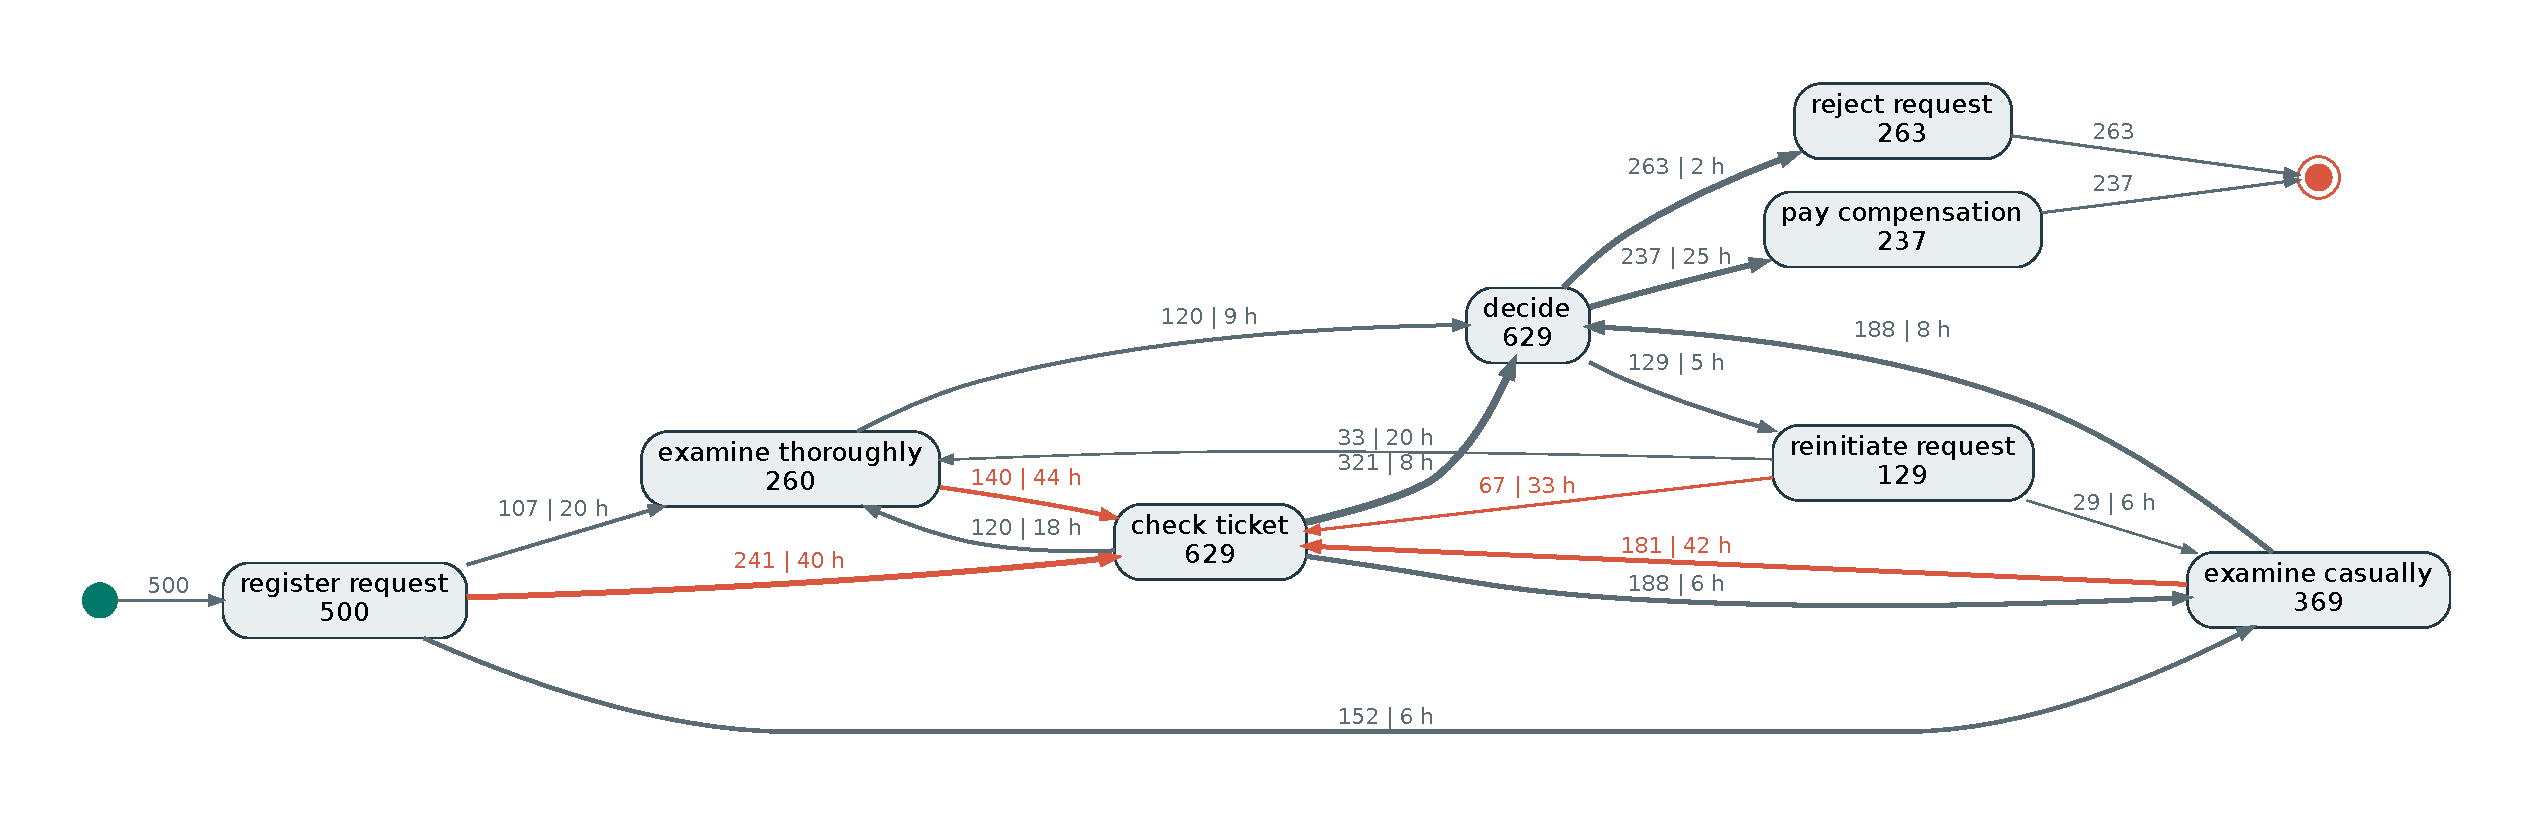
\includegraphics[width=\textwidth]{ch04/process_dfg}
\caption{Directly-follows graph of the compensation process. Nodes show the number of executions of each
activity; edges show the number of times the target directly follows the source and the mean time
between the two events. Edges slower than 30 hours are highlighted.}
\label{fig:dfg}
\end{figure}

\begin{figure}[htbp]
\centering
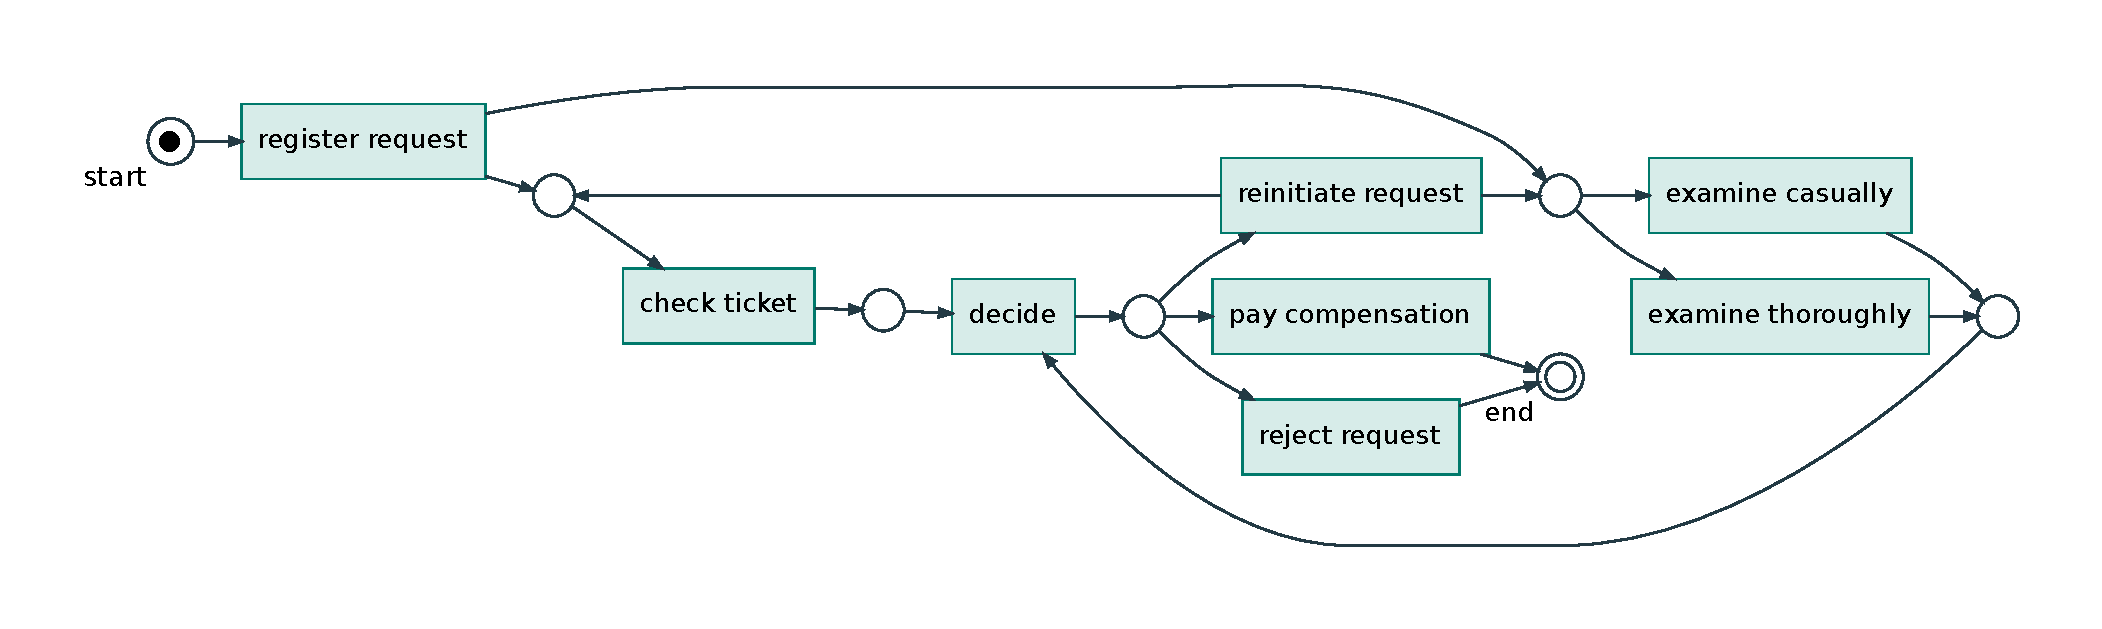
\includegraphics[width=0.92\textwidth]{ch04/process_petri}
\caption{Petri net discovered by the alpha algorithm. Boxes are transitions (activities), circles are
places; the token in the start place is the initial state.}
\label{fig:petri}
\end{figure}

The alpha algorithm is a clear introduction to process discovery, but it has well-known limitations:
it assumes that the log is complete and noise-free, and it cannot handle short loops or some
constructs. Practical algorithms, such as the heuristics miner \citep{weijters2006process}, which filters
infrequent behaviour, or the inductive miner \citep{leemans2013discovering}, which guarantees sound
models, are available in open-source tools such as ProM and PM4Py \citep{berti2019process}, and in
commercial products.

\subsection{Conformance checking}

Conformance checking\index{conformance checking} measures how well a model and a log agree. \emph{Token-based replay\index{token replay|textbf}}
\citep{rozinat2008conformance} plays each trace on the Petri net\index{Petri net}, firing the transition of each event: a
transition consumes a token from each of its input places and produces one in each of its output places.
If an input place is empty, the event did not respect the model, and a \emph{missing} token is created to
continue; tokens left in the net at the end are \emph{remaining}. With $p$, $c$, $m$ and $r$ the produced,
consumed, missing and remaining tokens over the whole log, the \emph{fitness\index{fitness|textbf}} is
\begin{equation}\label{eq:fitness}
  \mathrm{fitness}=\frac12\Bigl(1-\frac{m}{c}\Bigr)+\frac12\Bigl(1-\frac{r}{p}\Bigr),
\end{equation}
which is 1 when every trace can be replayed perfectly.

\begin{pylisting}[label={lst:conformance}]{Conformance checking by token-based replay}
from event_log import ACTIVITIES, simulate_log
from pm import alpha_miner, fitness, token_replay

code = {name: letter for letter, name in ACTIVITIES.items()}

def traces_of(log):
    log = log.sort_values(["case", "timestamp"])
    to_str = lambda s: "".join(code[a] for a in s)
    return list(log.groupby("case")["activity"].agg(to_str))

# the model is discovered from a clean log and checked against new cases
model = alpha_miner(traces_of(simulate_log(500, seed=0)))
for noise in (0.0, 0.1, 0.3):
    traces = traces_of(simulate_log(500, seed=1, noise=noise))  # new cases to check
    bad = [t for t in traces if token_replay(t, model)[2] > 0]  # missing tokens
    print(f"deviation rate {noise:.0%}: fitness {fitness(traces, model):.3f}, "
          f"{len(bad)} of {len(traces)} cases do not fit")
for t in bad[:2]:
    p, c, m, r = token_replay(t, model)
    print(f"case {t}: produced {p}, consumed {c}, missing {m}, remaining {r}")
\end{pylisting}
\begin{pyoutput}
deviation rate 0%: fitness 1.000, 0 of 500 cases do not fit
deviation rate 10%: fitness 0.987, 53 of 500 cases do not fit
deviation rate 30%: fitness 0.961, 155 of 500 cases do not fit
case abeg: produced 6, consumed 6, missing 1, remaining 1
case abedg: produced 7, consumed 7, missing 1, remaining 1
\end{pyoutput}

\Cref{lst:conformance} checks new cases against the net discovered from the clean log. Without deviations
the fitness is 1.000; when 10\% of the cases deviate (the ticket is not checked, or the decision is taken
before the examination or the check is finished) it falls to 0.987, and 53 of the 500 cases do not fit;
with 30\% of deviations, to 0.961, with 155 cases that do not fit. For the case $abeg$, which skips the
ticket check, the decision finds one of its input places empty (one missing token) and the token produced
for the check is never consumed (one remaining token): its own fitness is
$\frac12(1-\frac16)+\frac12(1-\frac16)=0.83$. Conformance checking tells the organisation how
often the rules are broken, which cases break them and where.

\subsection{Performance analysis}

Enriching the model with timestamps reveals where time is spent. In our log, the edges leading to the
ticket check take 40 to 44 hours on average, against roughly a day or less for the others (\cref{fig:dfg}). These are times between
consecutive recorded events: with completion events only, they mix service, waiting and the overlap of
concurrent activities (and our simple generator accumulates its timestamps sequentially, even where the
net allows concurrency), so they show where to look. They do not measure service durations. In this
simulation the ticket check is slow by construction, so speeding it up, or starting it earlier, would
shorten the whole process. Process mining\index{process mining} tools also
show the frequency of each variant, the workload of each resource, and the evolution of performance over
time, which links process mining with the monitoring\index{monitoring} of Unit~6.

% =====================================================================
\section{Robotic process automation}\label{sec:rpa}

\emph{Robotic process automation\index{robotic process automation (RPA)|textbf}} (RPA) tries to free people from the simple and repetitive tasks of
their daily work \citep{vanderaalst2018robotic,syed2020robotic}. It develops software agents, called
\emph{robots}, that mimic people performing business tasks on their computers: filling in forms,
processing the invoices received by e-mail, correcting mistakes in databases, copying data from one
application to another. RPA is widely adopted by companies and supported by vendors such as UiPath, Blue
Prism, Automation Anywhere and IBM. Its robots work through the same user interfaces as people, so they
can automate legacy systems that offer no programming interface, but they are brittle when the
interface changes.

\subsection{From RPA to intelligent process automation}

Most RPA\index{robotic process automation (RPA)} systems rely on explicitly encoded rules and configurations. Artificial intelligence
can extend these systems: \emph{intelligent process automation\index{intelligent process automation|textbf}} (IPA) aims to generalise RPA by
providing the tools to create complex workflows with minimal user intervention. The IEEE describes it as
a preconfigured software instance that combines business rules, experience-based context determination
logic and decision criteria to initiate and execute multiple interrelated human and automated processes
in a dynamic context \citep{ieee2017ipa}. A key step is the formalisation of workflows (the interaction
between the actions of the user, software and data artefacts) in a formal language that can be used to
simulate and execute them; the actions and events can be captured with tools that automate the graphical user interface (GUI), such as
Sikuli, which locates interface elements from screenshots \citep{yeh2009sikuli}. Discovering which
routines are worth automating from logs of user interactions is the goal of \emph{robotic process
mining\index{process mining|textbf}} \citep{leno2021robotic}, which brings together the two halves of this section.

\citet{ferreira2020evaluation} define IPA as a combination of four tasks between three representations of
a process (\cref{fig:ipa}): \begin{itemize}
\item \emph{Demo2text} describes in natural language a demonstration of a user
executing an activity; \item \emph{Demo2process} turns a demonstration into a program that can re-execute it;
\item \emph{Text2process} generates the process from a description of the activity, which is program synthesis
and inductive programming\index{inductive programming} (\cref{sec:indprog}); \item \emph{Process2text} describes in natural language a
process that is already implemented.
\end{itemize}

\begin{figure}[htbp]
\centering
\begin{tikzpicture}[font=\small\sffamily,
  rep/.style={draw=edmnavy,fill=edmnavy!6,rounded corners=3pt,minimum width=30mm,minimum height=10mm,align=center},
  arr/.style={-{Stealth[length=2.2mm]},edmteal,thick}]
  \node[rep] (demo) at (0,0) {demonstration\\(user actions)};
  \node[rep] (text) at (-3.4,-2.6) {natural language\\description};
  \node[rep] (proc) at (3.4,-2.6) {process\\(program)};
  \draw[arr] (demo) -- node[above left,text=edmnavy] {Demo2text} (text);
  \draw[arr] (demo) -- node[above right,text=edmnavy] {Demo2process} (proc);
  \draw[arr] ([yshift=2mm]text.east) -- node[above,text=edmnavy] {Text2process} ([yshift=2mm]proc.west);
  \draw[arr] ([yshift=-2mm]proc.west) -- node[below,text=edmnavy] {Process2text} ([yshift=-2mm]text.east);
\end{tikzpicture}
\caption{The four tasks of intelligent process automation \citep{ferreira2020evaluation}.}
\label{fig:ipa}
\end{figure}

\subsection{Two software robots}

In a visual RPA\index{robotic process automation (RPA)} tool such as UiPath, a robot is built by recording or assembling activities. A robot that
collects the prices of a product category from an online shop, for instance, is defined in five steps:
create a new process; open the web page of the category in the browser; select, with the data extraction wizard, one example of each field (the brand, the name and the price of a product); indicate the link to the next page,
so that the robot goes through all the pages; and add an activity that writes the extracted table to a CSV
file. From the examples of the third step, the tool infers the rest of the table, which is programming by example\index{programming by example} again. Then run it.

The same logic can be written in a few lines of code. \Cref{lst:rpa} is a robot that reads invoices
received by e-mail, extracts the supplier, the invoice number, the date and the amount, canonicalises
dates written in three formats and amounts written with European and English separators, and books the
invoices that pass the business rules. The cases it cannot handle, an invoice without a number and one
above the approval limit, are delegated to a person: as with the delegating\index{delegation} classifiers of
\cref{sec:cautious}, an automated system should recognise the cases it cannot handle. Each message is handled on its own, so an error in one does not stop the others; missing
fields, impossible dates (31 February) and unsupported amounts or currencies are delegated too, and the
output is written as proper CSV (the supplier ``Acme, SL'' contains a comma). The robot only prepares
records for booking: registering them in the accounting system is a separate step. Amounts are parsed only when they
match a declared format (European or English with two decimal places, or a plain integer): ambiguous amounts such as
12.480 or 12,3 are sent for human review, and the approval limit is applied to the canonical amount, never to a guessed
interpretation. The checks at the end of the listing are acceptance and rejection tests of this contract.

\begin{pylisting}[label={lst:rpa}]{A software robot that books invoices received by e-mail}
import csv
import re
import sys
from datetime import datetime
from decimal import Decimal, InvalidOperation

EMAILS = [  # the inbox the robot reads every morning
    "From: Ferreteria Sol\nSubject: Invoice INV-2041\nDate: 12/03/2026\n"
    "Total: 1.234,50 EUR",
    "From: Papeleria Mar\nSubject: Factura F-778\nFecha: 2026-03-15\nImporte: 89,90 EUR",
    "From: Tech Supplies Ltd\nSubject: Invoice no. 5531\nDate: 15 March 2026\n"
    "Amount due: EUR 12,480.00",
    "From: Limpiezas Turia\nSubject: Monthly service\nDate: 18/03/2026\n"
    "Total: 640,00 EUR",
    "From: Imprenta Rapida\nSubject: Factura F-2026-31\nFecha: 20/03/2026\n"
    "Total: 312,75 EUR",
    "From: Acme, SL\nSubject: Invoice INV-77\nDate: 31/02/2026\nTotal: 45,00 EUR"]
LIMIT = Decimal(10_000)                            # larger amounts need a manager

def parse_date(text):                              # None if impossible or unknown
    for fmt in ("%d/%m/%Y", "%Y-%m-%d", "%d %B %Y"):   # month names: English locale
        try:
            return datetime.strptime(text.strip(), fmt).date().isoformat()
        except ValueError:
            pass

FORMATS = {                                        # the only accepted amount formats
    "european": r"-?\d{1,3}(?:\.\d{3})+,\d{2}|-?\d+,\d{2}",     # 1.234,50  89,90
    "english": r"-?\d{1,3}(?:,\d{3})+\.\d{2}|-?\d+\.\d{2}",    # 12,480.00  89.90
    "integer": r"-?\d+"}                                       # 5

def parse_amount(line):
    """(amount, currency) if the whole field matches a declared format, else (None, None):
    ambiguous amounts such as 12.480 or 12,3 are never guessed."""
    cur = r"(EUR|USD|GBP)"
    m = re.fullmatch(rf"[^:]*:\s*(?:{cur}\s+)?(-?[\d.,]+)(?:\s+{cur})?\s*", line)
    if m is None or bool(m.group(1)) == bool(m.group(3)):     # exactly one currency
        return None, None
    number, currency = m.group(2), m.group(1) or m.group(3)
    if re.fullmatch(FORMATS["european"], number):
        number = number.replace(".", "").replace(",", ".")
    elif re.fullmatch(FORMATS["english"], number):
        number = number.replace(",", "")
    elif not re.fullmatch(FORMATS["integer"], number):
        return None, None
    return Decimal(number), currency

out = csv.writer(sys.stdout, lineterminator="\n")  # quotes fields when needed
out.writerow(["invoice", "date", "supplier", "amount", "status"])
for email in EMAILS:                               # every message is handled on its own
    supplier = re.search(r"From: (.+)", email)
    number = re.search(r"(?:Invoice|Factura)(?: no\.)? ([A-Z]+-[\d-]+|\d+)", email)
    date = re.search(r"(?:Date|Fecha): (.+)", email)
    date = parse_date(date.group(1)) if date else None
    amount, currency = parse_amount(email.splitlines()[-1])
    if number is None or supplier is None:
        status = "to human: no invoice number"
    elif date is None:
        status = "to human: missing or invalid date"
    elif amount is None or currency != "EUR" or amount <= 0:
        status = "to human: amount or currency not supported"
    elif amount > LIMIT:
        status = "to human: needs approval"
    else:
        status = "ready for booking"
    out.writerow([number.group(1) if number else "?", date or "?",
                  supplier.group(1) if supplier else "?",
                  f"{amount:.2f}" if amount is not None else "?", status])

print("\nformat checks (acceptance and rejection tests):")
for field in ["Total: 12.480 EUR", "Total: 12,3 EUR", "Total: 5 EUR",
              "Total: 1.234,50 EUR", "Total: 1,234.50 EUR", "Total: -1.234,50 EUR"]:
    amount, currency = parse_amount(field)
    print(f"  {field:22s} -> {'to human' if amount is None else f'{amount} {currency}'}")
\end{pylisting}
\begin{pyoutput}
invoice,date,supplier,amount,status
INV-2041,2026-03-12,Ferreteria Sol,1234.50,ready for booking
F-778,2026-03-15,Papeleria Mar,89.90,ready for booking
5531,2026-03-15,Tech Supplies Ltd,12480.00,to human: needs approval
?,2026-03-18,Limpiezas Turia,640.00,to human: no invoice number
F-2026-31,2026-03-20,Imprenta Rapida,312.75,ready for booking
INV-77,?,"Acme, SL",45.00,to human: missing or invalid date

format checks (acceptance and rejection tests):
  Total: 12.480 EUR      -> to human
  Total: 12,3 EUR        -> to human
  Total: 5 EUR           -> 5 EUR
  Total: 1.234,50 EUR    -> 1234.50 EUR
  Total: 1,234.50 EUR    -> 1234.50 EUR
  Total: -1.234,50 EUR   -> -1234.50 EUR
\end{pyoutput}

% =====================================================================
\section{Summary}\label{sec:summary4}

\begin{itemize}
  \item The steps of a data science project are automatable in very different degrees: modelling
        almost completely, data preparation and exploration partially, problem analysis and
        communication hardly at all.
  \item Data wrangling\index{data wrangling}, exploratory analysis and feature engineering\index{feature engineering} have many tools; deep feature
        synthesis\index{deep feature synthesis} generates features from relational data automatically.
  \item AutoML\index{AutoML} solves the combined algorithm selection\index{algorithm selection} and hyperparameter optimisation\index{hyperparameter optimisation} problem with
        random search\index{random search}, Bayesian optimisation\index{Bayesian optimisation}, multi-fidelity or evolutionary methods. The score of the
        selected configuration is optimistic, so the whole search must be evaluated on unseen data.
  \item Metalearning\index{metalearning} learns from previous experiments, for instance to select algorithms from
        meta-features; its value is bounded by how complementary the candidate algorithms are.
  \item Inductive programming\index{inductive programming} synthesises programs from examples and background knowledge\index{background knowledge}, in logic or
        functional languages; inductive bias\index{inductive bias} and domain-specific languages\index{domain-specific language} make the search tractable,
        and language models now act as few-shot inductive programmers.
  \item Large language models\index{large language model (LLM)} assist at every stage of a project and, as agents, carry out whole analyses;
        because their code can be plausible and wrong (hallucinated columns, leakage\index{data leakage}, silently dropped rows),
        it must be verified automatically: isolated execution, invariants and held-out evaluation.
  \item Genetic programming\index{genetic programming} evolves programs, represented as trees, by selection, crossover\index{genetic programming!crossover} and
        mutation\index{genetic programming!mutation}.
  \item Process mining\index{process mining} discovers, checks and enhances process models from event logs\index{event log}; robotic and
        intelligent process automation\index{intelligent process automation} build software robots that perform repetitive tasks.
\end{itemize}

\section*{Bibliographic notes}
\phantomsection\addcontentsline{toc}{section}{Bibliographic notes}

\citet{martinezplumed2021crisp} review data science processes from CRISP-DM\index{CRISP-DM} to data science trajectories.
\citet{hutter2019automated} is a standard reference on AutoML\index{AutoML}, and \citet{zoller2021benchmark} survey and
benchmark AutoML frameworks; \citet{brazdil2022metalearning} cover metalearning\index{metalearning} in depth.
\citet{gulwani2015inductive} present inductive programming\index{inductive programming} and its applications to end users, and
\citet{jaimovitch2023can} study language models for data wrangling\index{data wrangling}. \citet{debie2022automating} discuss what automating
data science\index{automated data science} means, and \citet{tornede2024automl} the opportunities and risks of large language models\index{large language model (LLM)} for AutoML. \citet{poli2008field} is a free field
guide to genetic programming\index{genetic programming}. \citet{vanderaalst2016process} is a reference book on process mining\index{process mining}, and
\citet{syed2020robotic} review the themes and challenges of RPA\index{robotic process automation (RPA)}.

\section*{Exercises}
\phantomsection\addcontentsline{toc}{section}{Exercises}

\begin{enumerate}[label=\textbf{4.\arabic*},ref=4.\arabic*,leftmargin=*,itemsep=6pt]
  \item\label{exr4:grid} A budget of nine evaluations is spent on two hyperparameters, only one of which
        matters. How many distinct values of the important hyperparameter does a $3\times3$ grid try? And
        random search\index{random search}?
  \item\label{exr4:ei} The best accuracy found so far is $f^\star=0.86$. A Gaussian process predicts
        $\mu=0.85$, $\sigma=0.02$ for configuration $z_1$ and $\mu=0.80$, $\sigma=0.06$ for $z_2$. Compute
        the expected improvement of both (\cref{eq:ei}). Which one is evaluated next, and why?
  \item\label{exr4:sh} Successive halving starts with 81 configurations, a budget $r$ each and $\eta=3$.
        How many configurations and what budget per configuration are there in each round? Compare the
        total budget with evaluating the 81 configurations with the final budget.
  \item\label{exr4:optimism} In \cref{lst:cash}, with 200 configurations the winner has a cross-validation
        accuracy of 0.950 and a test accuracy of 0.925. Explain the difference and design a protocol that
        gives an honest estimate of the performance of the AutoML\index{AutoML} process.
  \item\label{exr4:meta} Compute the following meta-features of a data set with 1000 examples, 20 features
        and classes of 900 and 100 examples: $\log_{10}n$, $\log_{10}d$, $n/d$, the minority fraction and
        the class entropy (in bits).
  \item\label{exr4:ilp} With the background predicates \texttt{parent/2}, \texttt{male/1} and
        \texttt{female/1}, write a clause for \texttt{grandmother(X,Y)}. How many literals does its body
        need, and why must it use a variable that does not appear in the head?
  \item\label{exr4:bias} How many sequences of $d=4$ functions can be formed with $b=5$ and with $b=20$
        background functions? How many ordered binary expressions with four operator nodes are there with
        those numbers of binary operators and three terminals (use $C_4=14$)? What does this tell you about
        the value of domain-specific languages\index{domain-specific language}?
  \item\label{exr4:pbe} With the DSL of \cref{lst:pbe}, write a program for the example
        \texttt{Ferri, Cesar} $\mapsto$ \texttt{C. Ferri}. Find the four shortest programs consistent with this single
        example and their outputs for \texttt{Garcia Lopez, Juan Jose}.
  \item\label{exr4:cross} In \cref{fig:gptrees}, which child results from replacing the leaf 3 of the second
        parent by the subtree $x\times x$ of the first?
  \item\label{exr4:alpha} Apply the alpha algorithm\index{alpha algorithm} to the log $L=\{abcd, acbd, aed\}$: compute the
        relations $\rightarrow$, $\parallel$ and $\#$ and the places of the Petri net\index{Petri net}.
  \item\label{exr4:replay} Replay the trace $abd$ on the net of Exercise~\ref{exr4:alpha} and compute its
        fitness\index{fitness}.
  \item\label{exr4:rpa} Classify each scenario as RPA\index{robotic process automation (RPA)} or IPA\index{intelligent process automation}: (a) a robot copies the fields of a web form
        into the accounting system following fixed rules; (b) a system watches an employee process a few
        claims and learns a program that processes new ones; (c) a system writes, from the code of a robot,
        a description of what it does for the auditors.
  \item\label{exr4:prompt} Write a few-shot prompt\index{prompt} that asks a language model to turn dates such as
        \texttt{23/12/2021} into \texttt{Dec 23, 2021}. How would you check the outputs before applying the
        transformation to a column of a million dates?
  \item\label{exr4:llmstage} Choose two stages of \cref{tab:llmstages}. For each, describe a task you would
        delegate to a language model assistant and an automatic check you would apply to its output.
  \item\label{exr4:verify} Which check of \cref{lst:assistant} catches each proposal? (a)
        \texttt{df["x"] = df["balance"] / df["limit"]} on a table without those columns; (b) the default rate of
        each customer's branch, computed on the whole table; (c) code that removes the customers with a missing
        income before computing a feature; (d) a feature that raises the cross-validated AUC by 0.001.
  \item\label{exr4:memorise} Without being given any training data, a language model predicts the survival of the
        Titanic passengers surprisingly well. Give two explanations, and say how you would evaluate its abilities
        fairly.
\end{enumerate}

\section*{Solutions to selected exercises}
\phantomsection\addcontentsline{toc}{section}{Solutions to selected exercises}

\begin{description}[font=\bfseries,leftmargin=0pt,itemsep=5pt]
  \item[\ref{exr4:grid}] The grid tries 3 values of each hyperparameter; random search\index{random search} tries 9 different
        values of each (with probability 1 for continuous ranges), so it explores the important one three
        times more finely.
  \item[\ref{exr4:ei}] For $z_1$, $u=-0.5$ and $\mathrm{EI}=0.02\,[-0.5\cdot0.3085+0.3521]=0.0040$. For $z_2$,
        $u=-1$ and $\mathrm{EI}=0.06\,[-1\cdot0.1587+0.2420]=0.0050$. The second point is evaluated: its mean is
        lower, but its uncertainty gives it a better chance of a large improvement (exploration).
  \item[\ref{exr4:sh}] Rounds of $81,27,9,3,1$ configurations with budgets $r,3r,9r,27r,81r$: each round costs
        $81r$, in total $405r$, against $81\cdot81r=6561r$, sixteen times more.
  \item[\ref{exr4:optimism}] The winner is the configuration with the highest cross-validation score among
        200, partly by luck, so its score is biased upwards. Evaluate the whole search with nested
        cross-validation\index{cross-validation!nested}, or run it on a training set and report the score of the final model on a
        separate test set that the search never uses.
  \item[\ref{exr4:meta}] $\log_{10}n=3$, $\log_{10}d=1.30$, $n/d=50$, minority fraction 0.1, and entropy
        $-0.9\log_20.9-0.1\log_20.1=0.469$ bits.
  \item[\ref{exr4:ilp}] \texttt{grandmother(X,Y) :- parent(X,Z), parent(Z,Y), female(X).} Three literals; the
        variable \texttt{Z}, the intermediate parent, connects $X$ and $Y$ and is not in the head.
  \item[\ref{exr4:bias}] Sequences: $5^4=625$ and $20^4=160{,}000$. Expressions: $C_4\,b^4\,3^5$, that is
        $14\cdot625\cdot243=2{,}126{,}250$ and $14\cdot160{,}000\cdot243=544{,}320{,}000$. The count depends on the
        grammar, but in every case a small, specialised set of functions keeps the space small enough to
        search, which is what DSLs\index{domain-specific language} provide.
  \item[\ref{exr4:pbe}] The program \texttt{initial(word,1)} + \texttt{". "} + \texttt{token(word,0)}. Eight programs are consistent with the example. The four shortest combine
        \texttt{initial(word,1)} or \texttt{initial(word,-1)} with \texttt{token(word,0)} or
        \texttt{token(word,-2)}; for the new input they give \texttt{L. Garcia}, \texttt{L. Juan},
        \texttt{J. Garcia} and \texttt{J. Juan}. The other four are longer variants that split the separator \texttt{". "} into two
        constants and behave in the same way. The intended answer (\texttt{J. Garcia}) needs more examples,
        or a richer DSL.
  \item[\ref{exr4:cross}] $xy-x^2$.
  \item[\ref{exr4:alpha}] $a\rightarrow b$, $a\rightarrow c$, $a\rightarrow e$, $b\rightarrow d$, $c\rightarrow d$,
        $e\rightarrow d$, $b\parallel c$, and $a\#d$, $b\#e$, $c\#e$ (pairs that never directly follow each
        other: $a$ and $d$ appear in every trace, so $\#$ does not mean exclusive choice). Places: $(\{a\},\{b,e\})$, $(\{a\},\{c,e\})$,
        $(\{b,e\},\{d\})$, $(\{c,e\},\{d\})$, plus the source place before $a$ and the sink place after $d$.
  \item[\ref{exr4:replay}] $a$ consumes the start token and produces two; $b$ consumes one and produces one;
        $d$ needs tokens in $(\{b,e\},\{d\})$, present, and $(\{c,e\},\{d\})$, missing; finally the end token is
        consumed. $p=5$, $c=5$, $m=1$, $r=1$ (the token for $c$), so the fitness\index{fitness} is
        $\frac12(1-\frac15)+\frac12(1-\frac15)=0.8$.
  \item[\ref{exr4:rpa}] (a) RPA\index{robotic process automation (RPA)}. (b) IPA\index{intelligent process automation} (Demo2process). (c) IPA (Process2text).
  \item[\ref{exr4:prompt}] For instance: \texttt{input: 23/12/2021, output: Dec 23, 2021; input: 05/01/2022,
        output: Jan 5, 2022; input: 31/07/2023, output:}. Check the outputs on held-out examples with known
        answers, validate their format with a regular expression, and compare the parsed dates with the
        inputs (same day, month and year) before trusting the transformation.
  \item[\ref{exr4:llmstage}] For example, data preparation: ask for the code that standardises the dates of a
        column, and check that the number of rows is unchanged and that the result matches a few dates converted by
        hand. Modelling: ask for a pipeline, and check that the preprocessing is fitted inside the cross-validation
        and that the model beats a simple baseline on held-out data.
  \item[\ref{exr4:verify}] (a) Running the code: the columns do not exist (a hallucination). (b) Running it without the
        target: the default rate uses the target (leakage\index{data leakage}). (c) The invariant on the rows. (d) The minimum gain: an
        improvement of 0.001 is within the noise of cross-validation.
  \item[\ref{exr4:memorise}] The data set is very likely in its training data, so it may have memorised it
        (contamination\index{contamination of benchmarks}); and texts about the Titanic describe its patterns (women and children first, the classes of the
        cabins). A fair evaluation uses data the model cannot have seen, such as recent or private data, or a perturbed
        version of the data set, and compares the model with a classifier trained on the same information.
\end{description}

